% % % % % % % % % % % % % % % % % % % % % % % % % % % % % % % % 
% =========================================================== %
% % % % % % % % % % % % % % % % % % % % % % % % % % % % % % % %
\chapter{Corrections and Changes Made}
\label{ch:corr}
% % % % % % % % % % % % % % % % % % % % % % % % % % % % % % % % 
% =========================================================== %
% % % % % % % % % % % % % % % % % % % % % % % % % % % % % % % %

In the following list of changes made, the section numbers and page numbers refer to the original
text as quoted in the correction sheet and could have changed in the latest version of the text.

Version Info:
\begin{itemize}
 \item v1: Initial version
 \item v2: Mairi's Point 15 and Kazuya's Point 8 on analytic solutions added.
 \item v3: Mairi's Point 12 and Kazuya's Point 6 on initial conditions revised.
\end{itemize}


\section{Mairi's Corrections}

\subsection{Point 1: Short corrections}
\textbf{The changes have been made. 
In the case of one of the corrections the notation $K_1,K_2,K_3$ was to be changed to
$k_1,k_2,k_3$. However the $K_i$ as used refer to the range of $k$ values in the simulation and
not to individual $k_i$ values so this has not been changed.}

\subsection{Point 2: Drawbacks of Inflation}
\textbf{Added to discussion on Pg 36:}

In this thesis inflation is taken to be the mechanism by which inhomogeneities in matter are seeded
and the horizon and flatness problems of the Big Bang are solved. However, the inflationary
paradigm is not without its own challenges.

Chief amongst these is the lack of a unique underlying theory. Many high energy theories have been
shown to produce an inflationary phase. Often, however, these require a great deal of fine-tuning
in order to produce a sufficient number of e-foldings of inflation. Lack of knowledge about the
governing physics at high energy scales hampers our understanding of the cause of inflation and
undermines any analysis of the generic nature of the initial conditions required.

The overall duration of inflation is also unknown. Observations only require that currently
observable scales were previously inside the horizon. Thus the onset of inflation is not
constrained and could occur far in the past. However, allowing such a long inflationary period
typically increases the fine-tuning necessary and can lead to other issues. 

There are further problems with the inflationary paradigm, including the lack of an explanation for
how energy in the inflaton field is transferred to the other constituent parts of the universe, and
indeed the fact that no scalar field has yet been directly observed.

We will continue to employ the inflationary paradigm in this thesis but it is important to
acknowledge that some challenges remain to be overcome.

\subsection{Point 3: T-duality discussion}
\textbf{Inserted on Pg 40 just below Section 3.2.2 header:}

In string theory an extra space time symmetry is present which relates physical properties in
theories with large compactification radius with those in theories with small radius. 
Suppose we have a string theory compactified on a circle of radius $L$. The ``T-duality''
transformation which relates two physical theories with this one compactified dimension is
% 
\begin{equation}
\label{eq:tdualtransform-corr}
 L \rightarrow \wt{L} = \frac{\alpha'}{L}\,.
\end{equation}
% 
Now consider what effect this transformation will have on the momentum of a closed string. Instead
of being a continuum, the momentum takes discrete values \ldots
\\

\textbf{Rephrased end of Section 3.2.2 on Pg 41 as follows:}

The formula for the mass spectrum, \eq{eq:closedmass-dbiintro}, is invariant
when $j$ and $w$ are exchanged given the transformation in \eq{eq:tdualtransform-dbiintro}.
Writing the equations of motion in terms of $\wt{L}$, having interchanged $j$ and
$w$, gives a new theory which is compactified on a circle of radius $\wt{L}$. This is known as the
T-dual theory \cite{Sakai1986,Kikkawa1984b}. The two
theories are physically identical since T-duality is an exact symmetry
of string theory for closed strings. The T-duality applies to all physics in the theory and in
particular also affects open string modes. These behave in a different way under T-duality to closed
strings as will be described below.
\\

\textbf{Rephrased part of Section 3.2.3 on Pg 41 as follows:}

We introduced T-duality by explaining
its effects on closed strings. But what happens to the open strings in a T-dualised theory? Open
strings, as their name suggests, have two open ends and
consequently cannot have a conserved winding number such as $w$. Suppose once more
that one
of the $D$ dimensions is compactified. As $L\rightarrow0$, the non-zero momentum
states become infinitely massive, but in contrast to the closed case there is now
no continuum of winding states. Thus, the open string now lives in $D-1$ dimensions
similar to the result of standard KK compactification \cite{Johnson2000}.
The endpoints of the open strings 
then observe Dirichlet boundary conditions, taking fixed values in the compactified
direction.
There are still closed strings in this theory, however, and these continue to
move in the full $D$ dimensions after being T-dualised.  

The result is similar if more than
one coordinate is made periodic.
If $D-p-1$ spatial dimensions are compactified, for some $p$, then the ends of
the open
strings can still move freely in the other $p$ spatial dimensions on a $p+1$
dimensional hypersurface. This hypersurface is called a Dirichlet brane or
D$p$-brane. The closed string modes move in the full $D$ dimensions.



\subsection{Point 4: Validity of Eq 3.28}
\textbf{Added to end of Pg 48:}

In deriving \eq{eq:approxlyth-dbiintro} we have assumed that $r/\cs \PX$ varies slowly during
observable inflation. For the DBI case, $\cs \PX = 1$ and the change in $r$ can be related to the
change in $\epsilon_H$ and $\cs$ through \eq{eq:rdefn-dbiintro}. As we have taken $\epsilon_H,
|\eta_H|,|s|\ll 1$ the tensor-scalar ratio will indeed vary slowly over the observable epoch.
% 
For more general models where $\cs \PX \ne 1$ we have that
% 
\begin{equation}
 \frac{\d }{\d \N}\left[ \frac{r}{\cs \PX}\right] = 16\frac{\epsilon_H}{\PX}\left( 2\epsilon_H
-2\eta_H\right)\,.
\end{equation}
% 
Therefore $r/\cs\PX$ varies slowly as long as $\PX$ is not too small, \iec close to
$\mathcal{O}(\epsilon_H^2)$. This will not be the case in the models studied in Chapters
\ref{ch:dbi} and \ref{ch:multibrane}.

\subsection{Point 5: No isocurvature mode considered}
\textbf{Added to Perturbation section on Pg 24:}

For single field models no mixing
of adiabatic and non-adiabatic modes occurs \cite{Weinberg200804}. Therefore, throughout this
thesis we will only consider adiabatic perturbations and ignore any isocurvature mode present.

\subsection{Point 6: Assumptions leading to \texorpdfstring{$r<10^{-7}$}{r<10**-7}}
\textbf{Added to Section 4.2 on Pgs 54 and 55:}


Before concluding this section, we should explicitly outline all the assumptions that have lead to
\eq{eq:standardbound}. First, we are considering the relativistic limit where $\cs\ll1$. We are
also restricting ourselves to considering the UV scenario where a brane moves towards the tip of
the throat. This ensures that \eq{eq:importantbound} is satisfied. For the Lyth bound to take the
form in \eq{eq:approxlyth-dbiintro}, we have assumed that $r$ varies slowly during the observable
period of inflation. This is justified as the change in $r$ can be written in terms of the
quasi deSitter parameters $\epsilon_H, \eta_H$ and $s$ and we have assumed their magnitudes are
much less than unity.
\\
\ldots
\\
In order to neglect the $\fnleq$ term in \eq{eq:boundpower6} we have assumed that $-\fnleq>5$. As
$\cs$ has been taken to be small this is expected to be the case. The volume of the Sasaki-Einstein
manifold $X_5$ is taken to be $\mathcal{O}(\pi^3)$ in keeping with the values for known solutions.
The WMAP5 normalisation of the scalar perturbation power spectrum has also been used. Finally, in
going from \eq{eq:upperbound} to the final numerical figure in \eq{eq:standardbound} the most
``optimistic'' value, $\Delta \N_*\simeq 1$, has been chosen as this leads to the least
restrictive bound on $r$.  As described above a more realistic value of $4$ would severely
constrain $r$ due to the strong dependence of \eq{eq:upperbound} on $\Delta\N_*$.

\subsection{Point 7: Discussion of \texorpdfstring{$Y^{p,q}$}{Y**p,q}}
\textbf{Added to Section 4.3 on Pg 57:}

Previously only two five-dimensional Sasaki-Einstein
metrics were explicitly known, $S^5$ and $T^{1,1}$ on $S^2\times S^3$. The $Y^{p,q}$ metrics
described in \Rref{gauntlett} are a countably infinite number of Sasaki-Einstein metrics on
$S^2\times S^3$. The metrics are parametrised by the two topological numbers $p$ and $q$, which are
coprime when the $Y^{p,q}$ is topologically $S^2\times S^3$. The volume of one of these manifolds
is proportional to $1/p$. Hence by setting $q=1$ and letting $p$ become large, this volume can be
made arbitrarily small \cite{gauntlett}. On the other hand, the largest volume occurs for $p=2$,
$q=1$ giving $\mathrm{Vol}(Y^{2,1})\simeq 0.29\pi^3$. 

\subsection{Point 8: Rewrite Section 4.4 more clearly}
\textbf{Many changes have been made to Section 4.4 including splitting the later parts into two
subsections. The functions $f_1$, $f_2$ and $f_3$ have been renamed $f_A$ etc in order to avoid
confusion with Section 5.2. Many equations from previous sections have been repeated in order to
improve readability.}

\textbf{Major changes:}

\textbf{Change to introductory section on Pg 58:}

In this section, we take a phenomenological 
approach and consider the following kinetic function which has a more general form than the DBI one
but still contains a square root term:
% 
\begin{equation}
\label{eq:genaction-corr}
P= -f_A (\varphi ) \sqrt{1-f_B (\varphi ) X} -f_C (\varphi) \,,
\end{equation}
% 
where $f_i (\varphi )$ are unspecified functions of the inflaton 
field. We will assume 
implicitly that these functions have a suitable form for 
generating a successful phase of inflation.
A direct comparison with \eq{eq:Pdefn-dbiintro} 
indicates that the standard DBI action can be recovered by setting $f_A f_B =2$. This implies
that $\cs P_{,X} =1$ and greatly simplifies the form of \eq{eq:rtheory}. 
Another important property in the DBI case is that the warp factor uniquely determines 
the kinetic structure of the action, i.e., $h^4 \propto f_A \propto f_B^{-1}$.  
In view of this, it is interesting to consider whether
the gravitational wave constraints could be weakened by relaxing one 
or both of these conditions. 

% 
% \eq{eq:genaction-dbi} 
% can be transformed into a similar form to that of 
% \eq{eq:Pdefn-dbiintro} through the field redefinition 
% % 
% \begin{equation}
% \label{eq:defvarphi}
% \tilde{\varphi} \equiv \int d \varphi \sqrt{\frac{f_Af_B}{2}}  \,.
% \end{equation}
% 

We can differentiate $P(X, \vp)$ in \eq{eq:genaction-dbi} to find:
% 
\begin{align}
 \PX &= \frac{f_A f_B}{2\sqrt{1-f_B X}} \,, \\
 P_{,XX} &= \frac{f_A f_B}{2}\frac{f_B}{2(1-f_B X)^{\frac{3}{2}}} \,.
\end{align}
% 
% 
The sound speed of fluctuations in 
the inflaton, defined in \eq{eq:defcs-dbiintro}, is then given by
%  
\begin{equation}
\label{eq:cs-corr}
\cs = \sqrt{1-f_B X} = \frac{f_Af_B}{2} \frac{1}{P_{,X}}  \,,
\end{equation}
% 
and the scalar power spectrum \eqref{eq:Ps-dbiintro} by
% 
\begin{equation}
\label{eq:spectrum-corr}
\Pr = \frac{1}{2\pi^2}\frac{H^4}{f_Af_B\dot{\varphi}^2}  \,.
\end{equation}

\textbf{Explanation of generalisation of BM bound on Pg 59 expanded and revised:}

The BM bound \eqref{eq:BMboundr} restricts the maximal 
variation of the scalar field $\varphi$ in the full throat region for DBI inflation. 
This is determined by expression \eqref{eq:BMbound-dbi} 
for generic warped geometries that are asymptotically 
$AdS_5 \times X_5$ away from the tip of the throat. However, in Section~\ref{sec:lyth-dbiintro} the
Lyth bound was also defined for general
non-canonical actions. For the more general kinetic function
\eqref{eq:genaction-dbi}, the BM bound becomes
% 
\begin{equation}
\label{eq:bmboundgen-corr}
 r < \frac{32}{N(\Neff)^2}\cs\PX = \frac{16}{N(\Neff)^2}f_A f_B \,.
\end{equation}
% 
To use this bound we must be able to calculate $\Neff$ over the full range of e-foldings of
inflation. This requires knowledge of the behaviour of $f_A$ and $f_B$ over that range. 

A more cautious approach would be to restrict our attention to 
the observable stage of inflation.
Assuming that the variation
of $f_Af_B = 2 \cs\PX$ is negligible during that epoch, we can use
\eq{eq:approxlyth-dbiintro} which states that 
% 
\begin{equation}
\label{eq:genphivary1-corr}
\left( \frac{\Delta \varphi}{\Mpl} \right)^2_{*} \simeq 
\frac{(\Delta \N_{*} )^2}{8} \left(\frac{r}{\cs\PX}\right)_*  
= \frac{(\Delta \N_{*} )^2}{4} \left(\frac{r}{f_A f_B}\right)_*  \,.
\end{equation}
% 
In addition, 
if observable scales leave the horizon 
while the brane is inside the throat, the change in the field value 
must satisfy $| \Delta \varphi_*|<\varphi_{UV}$. It follows from \eqs{eq:bmboundgen-dbi} and
\eqref{eq:genphivary1}, therefore, that 
% 
\begin{equation}
\label{eq:genBMbound-corr}
r_*< \frac{32}{N (\Delta \N_{*})^2} (\cs\PX)_* = \frac{16}{N (\Delta \N_{*})^2}
(f_Af_B)_* \,.
\end{equation}
% 

Condition 
(\ref{eq:genBMbound}) will be referred to as the 
generalised BM bound. 
We have been
conservative by restricting our discussion to the 
observable phase of inflation. A stronger condition is obtained by using
\eq{eq:bmboundgen-dbi}, which is equivalent to substituting $\Delta \N_* \rightarrow 
\Neff$. If 
$f_Af_B$ remains nearly constant over the last $\N$ 
e-foldings of inflation, 
then $\Neff$ may be as large as $60$ and the right hand side of \eq{eq:genBMbound} will be reduced
by a factor of $225$. 
Thus, the generalised bound 
(\ref{eq:genBMbound}) should be regarded as a necessary 
(but not sufficient) condition to be satisfied by the tensor modes.


\subsection{Point 9: Naturalness of multi-coincident brane inflation}
\textbf{Added to Section 5.1 on Pg 65:}

One scenario in which multiple branes are expected is after brane flux annihilation, in which
branes travelling down the throat annihilate with the trapped flux, creating new branes
\cite{thomasward, DeWolfe:2004qx, Kachru:2002gs}. These are then attracted by other branes and
fluxes in other throats and propagate toward the bulk.
In \Rref{thomasward} Thomas \& Ward argue that it is unlikely that only a single brane is left
after the flux annihilation process, due to the large amount of fine tuning necessary to achieve
this. Instead it is more likely that a number of branes remain.

\subsection{Point 10: Rephrasing of Section 5.4 about large n limit}
\textbf{Two subsection headers have been inserted and the main bulk of Section 5.4 has been
rephrased. A factor of 2 error has been fixed but conclusions remain the same.}

\textbf{Reworked section:}

The regime $W \gg 1$ is of interest for 
relaxing the gravitational wave constraints\footnote{Note that 
the case $n \gg 1$ and
$W \sim 1$ will not significantly relax the BM bound, 
since we require $n \ll N$ for backreaction effects to be negligible.}. 
The generalised BM bound for IR models, with branes propagating towards the bulk, is given by 
\eq{eq:f2IRlower}:
% 
\begin{equation}
\label{eq:f2IRlower-corr}
\frac{f_2\Mpl^4}{N} > \frac{(\Delta \N_*)^2}{4\pi^2}
\frac{\sqrt{-3\fnleq}}{(1-n_s)\Pr}  \,.
\end{equation}
% 
As we know $f_2$, this may be expressed as 
a limit on the value of the warp factor $h(\varphi_*)$ on CMB scales: 
% 
\begin{equation}
\label{eq:warptorelax-corr}
N T_3 \left(\frac{h_*}{\Mpl}\right)^4 < 
\frac{8\pi^2 (1-n_s)\Pr}{\sqrt{-3\fnleq}(\Delta \N_*)^2} \,.
\end{equation}
% 


We now consider whether this limit can be satisfied for reasonable choices 
of parameters when the warped compactification corresponds to 
an $AdS_5$ or KS throat, respectively. Recall that the warp 
factor for the $AdS_5$ throat is given by $h=\varphi/(\sqrt{T_3}L)$.  
Condition (\ref{eq:warptorelax}) therefore reduces to a constraint on the 
value of the inflaton during observable inflation: 
% 
\begin{equation}
\label{eq:phivalue-corr}
\frac{\varphi_*^4}{\Mpl^4} < 
\frac{8\pi^2 (1-n_s)\Pr}{\sqrt{-3\fnleq} ( \Delta \N_*)^2} 
\frac{T_3 L^4}{N} \,.
\end{equation}
%  
However, non-perturbative string effects are expected to become 
important below a cutoff scale, $\varphi_{\rm cut} = 
h_{\rm cut} \sqrt{T_3} L$, where $h_{\rm cut}$ is the value of the 
warp factor at that scale. For consistency, therefore, one requires 
$\varphi_*>\varphi_{\rm cut}$, so that 
% 
\begin{equation}
 N T_3 \left(\frac{h_\mathrm{cut} }{\Mpl}\right)^4 < 
\frac{8\pi^2 (1-n_s)\Pr}{\sqrt{-3\fnleq} ( \Delta \N_*)^2} \,,
\end{equation}
% 
which implies an upper limit on the 
${\rm D3}$-brane charge: 
% 
\begin{equation}
\label{eq:Nlimit-corr}
N< \frac{64\pi^5 \gs (1-n_s)\Pr}{\sqrt{-3\fnleq} ( \Delta \N_*)^2}
\left( \frac{\Mpl}{h_{\rm cut} \ms} \right)^4   \,.
\end{equation}
% 
Assuming the typical values $\ms \sim 10^{-2}\Mpl$, 
$\Delta \N_* \simeq 4$ and 
$h_{\rm cut} \sim 10^{-2}$ implies
%   
\begin{equation}
N < 1.76 \times 10^8 (1-n_s)(-\fnleq)^{-1/2} \,, 
\end{equation}
% 
and for $1-n_s <0.05$ and $-\fnleq>5$ the inequality becomes
% 
\begin{equation}
 N < 4\times 10^6\,.
\end{equation}
%  


For an $AdS_5$ throat, the fuzzy potential $W$ is a constant,
and the condition that $W \gg 1$ becomes 
% 
\begin{equation}
\label{eq:Chatlimit-corr}
\hat{C} \ll \frac{4\pi^2\gs N}{\mathrm{Vol}(X_5)} \,.
\end{equation}
% 
Hence, combining inequalities 
(\ref{eq:Nlimit-dbi}) and (\ref{eq:Chatlimit}) implies that
%  
\begin{equation}
\label{eq:nlimit-corr}
\hat{C} \ll 
\frac{2 (2\pi)^7 (1-n_s)\Pr}{\sqrt{-3\fnleq} ( \Delta \N_*)^2}
\frac{\gs^2}{\mathrm{Vol} (X_5) }
\left( \frac{\Mpl}{h_{\rm cut}\ms} \right)^4  \,,
\end{equation}
% 
and specifying $\gs \sim 10^{-2}$ and 
$\mathrm{Vol}(X_5) \simeq \pi^3$ then yields the limit  
% 
\begin{equation}
\hat{C} \ll 2.25\times 10^{6} (1-n_s)(-\fnleq)^{-1/2} < 5\times 10^4,
\end{equation}
% 
 or equivalently,
%   
\begin{equation}
\label{eq:nbound-corr}
n \ll 225.
\end{equation}
% 
In deriving the action \eqref{eq:largeP-multi} the number of coincident branes was assumed to be
large. However we have now found that for the case of branes propagating towards the bulk, the
number of such branes is bounded from above.
Furthermore, since $f_1f_2 \simeq {\rm constant}$ for the $AdS_5$ throat, 
the stronger form of the inequality (\ref{eq:genBMbound}) may be used. The right hand side of
inequality \eqref{eq:nlimit-dbi} would be reduced by a factor of $(   \Neff /\Delta \N_*)^2$ by
substituting 
$\Delta \N_* \rightarrow \Neff$. This ratio 
could be as high as $(60/4)^2 \simeq 200 $, leading to $n$ being less than $15$. In this case
the assumption of large $n$ would clearly be inconsistent and the model would be ruled out. 

\subsection{Point 11: Changed ``hybrid'' to ``toy model''}
\textbf{All mentions of the hybrid model have been changed.}

\textbf{Change in list of models on Pg 102:}
\begin{enumerate}
\item[4.] $V(\vp) = \msqphisqwithV$. This is a contrived toy model which requires inflation to
be terminated by hand. We will set inflation to end when $\vp \simeq 8$. By taking a value
of $U_0 = 5\e{-10}\Mpl^{4}$ a blue spectrum ($n_s>1$) can then be obtained
\cite{Linde:1993cn,Komatsu:2008hk}.
\end{enumerate}

\textbf{Change in description on Pg 129:}
The fourth model, with potential $V(\vp)=\msqphisqwithV$, is a contrived toy model.
As described in Section~\ref{sec:pots-num}, in order to perform the single field
calculation, the end time of inflation must be specified by hand. 

\textbf{Change in caption of Fig 8.12 on Pg 131:}
Comparison of the
source term
evolution for the four different models. After horizon crossing the magnitude of the
source term is larger for the quadratic and quartic models than for the other two.
Towards the end of the numerical calculation there is a marked increase in $|S|$ for
three of the models as $\bar{\varepsilon}_H$ increases towards unity. The end time of
inflation is specified by hand for the contrived toy model, so this effect is
not seen.

\subsection{Point 12: Initial Conditions}
\textbf{REVISED in v3: The initial conditions for the second order perturbations are set in Section 7.2.2 on Pg
105. It was suggested that these conditions introduce a homogeneous solution into the
final solution for $\dvp2$ as shown in Fig 8.2. I have looked at trying to remove this solution
numerically but think that a full recalculation and analysis cannot be undertaken in the time available.
The references to a zero homogeneous solution have been removed and the discussion in Section 7.2.2 amended
to reflect this. The derivation of the analytic homogeneous solution which was added as
Appendix~\ref{sec:init-apx}, has been changed to the following:}

The homogeneous equation for the second order perturbations is  
% 
\begin{equation}
\label{eq:homogen-corr}
 \dvp2''(\eta, \kvi) + 2\H \dvp2'(\eta, \kvi) 
+ \left[ k^2 + a^2\Upp - 24\pi G (\vp_0')^2 \right]\dvp2(\eta,\kvi) = 0\,.
\end{equation}
% 
During slow roll, with the slow roll variables $\varepsilon_H$ and $\eta_H$ defined in
Chapter~\ref{ch:introduction}, this becomes
% 
\begin{equation}
 \dvp2'' + 2\H \dvp2' + \left[k^2 + 3\H^2(\eta_H + \varepsilon_H)\right]\dvp2 = 0\,.
\end{equation}
% 
If we let $u=a\dvp2$, this equation can be rewritten as
% 
\begin{equation}
\label{eq:uH-corr}
 u'' + \left[k^2 +\H^2(3\eta_H - 2\varepsilon_H - 2)\right]u = 0\,.
\end{equation}
% 
When $\varepsilon_H$ is small, the conformal time $\eta$ is given by 
% 
\begin{equation}
 \eta \simeq -\frac{1}{\H(1-\varepsilon_H)}\,,
\end{equation}
% 
so we can rewrite \eq{eq:uH-corr} as
% 
\begin{equation}
 u'' + \left[k^2 + \frac{1}{(-\eta)^2}\frac{3\eta_H -2\varepsilon_H -2}{(1-\varepsilon_H)^2} 
       \right]u = 0\,.
\end{equation}
% 
If the derivatives are taken in terms of $(-\eta)$ instead of $\eta$ this is in the form of a
Bessel equation with solutions in terms of Hankel functions given by
% 
\begin{equation}
 u_{1,2} = \sqrt{-\eta} H_\nu^{(1,2)}(-k\eta)\,, 
\end{equation}
% 
where $H_\nu^{(1,2)}$ are the Hankel functions (Bessel functions of the third kind), and $\nu$ is
given by
% 
\begin{equation}
 \nu^2 = \frac{6\varepsilon_H -12\eta_H + 7}{4(1-2\varepsilon_H)}\,.
\end{equation}
%

The full solution for $u$ is then
% 
\begin{equation}
 u_\mathrm{full} = C_1 \sqrt{-\eta} H_\nu^{(1)}(-k\eta) +
                   C_2 \sqrt{-\eta} H_\nu^{(2)}(-k\eta)\,,
\end{equation}
% 
where $C_1, C_2\in \mathbb{C}$. When the (real) argument of the Hankel functions goes to $+\infty$
they have the following asymptotic form \cite{abramowitz+stegun}:
% 
\begin{align}
 H_\nu^{(1)}(z) &\rightarrow \sqrt{\frac{2}{\pi z}} e^{i(z-\frac{\pi}{2}\nu - \frac{\pi}{4})} \,,\\
 H_\nu^{(2)}(z) &\rightarrow \sqrt{\frac{2}{\pi z}} e^{-i(z-\frac{\pi}{2}\nu - \frac{\pi}{4})} \,.
\end{align}
% 

So at early times when $\eta\rightarrow -\infty$ and $-k\eta\rightarrow +\infty$ we have the
following expressions for u:
% 
\begin{align}
 u_{i} &= \sqrt{\frac{2}{\pi k}}\left( C_1 e^{-i(k\eta +\frac{\pi}{2}\nu + \frac{\pi}{4})}
                + C_2 e^{+i(k\eta +\frac{\pi}{2}\nu + \frac{\pi}{4})} \right) \,,\\
 u_{i}' &= i k\sqrt{\frac{2}{\pi k}}\left( -C_1 e^{-i(k\eta +\frac{\pi}{2}\nu + \frac{\pi}{4})}
                + C_2 e^{+i(k\eta +\frac{\pi}{2}\nu + \frac{\pi}{4})} \right) \,,\\
\end{align}
% 
where we have assumed that $\nu$ is slowly varying far in the past, \iec the derivatives of the slow
roll parameters are very small.

As explained in Section~\ref{sec:initconds-num}, the results given for $\dvp2$ are for the full solution
including the homogeneous part. To remove the homogeneous part of the solution the initial conditions
for the full $\dvp2$ should be chosen such that $C_1=C_2=0$ at all times. 

\textbf{REVISED in v3: The note added to the main text in Section~7.2.2 on Pg 106 (Pg 113 in new version)
has been changed to the following:}

%  
We are interested in the production of second order effects by the
evolution of the the Gaussian first order modes and we make no
assumptions about the existence of second order perturbations before
the simulation begins. Therefore, we set the initial condition for each second order
perturbation mode to be $\dvp2=0, \dN{\dvp2}=0$ at
the time when the corresponding first order perturbation is initialised.
One argument in favour of this choice of initial conditions is that far in the past the perturbations
are assumed to be Gaussian and therefore the second (and higher) order perturbations would be identically zero. 
% 

A numerical solution for the second order perturbation equation will contain a homogeneous solution
and a particular solution. 
The homogeneous part of the solution of
the slow roll equation, \eq{eq:KG2-fourier-sr-ntime}, can be calculated analytically 
as done in Appendix~\ref{sec:init-apx}. On their own the initial conditions we have chosen above do not  
remove this homogeneous solution from the result for $\dvp2$ in general. In order to do this, and keep only the 
particular solution to the equation, it is necessary to ensure that the homogeneous solution is the trivial $(0,0)$ 
solution throughout the evolution. We have not attempted to do this in this thesis but it is an important
issue for further study in the future. Approaches to removing the homogeneous part of the solution include
calculating a semi-analytic value for the second order initial conditions which equals the particular solution
 or numerically trying to select the trivial
homogeneous solution by introducing a ramping function to the source term in \eq{eq:KG2-source-ntime}.
In summary, the results quoted in Chapter~\ref{ch:results} for the second order perturbations include both a homogeneous 
and particular solution. Extraction of either of these parts from the full result remains an issue for future study.

\subsection{Point 13: Move some calculations into an appendix}
\textbf{Three large sections of calculations have been moved into the appendix.}

\textbf{All of Section 5.2.2 on Pg 68 has been moved to Appendix~\ref{sec:apx-multi}.}

\textbf{A part of Section 5.5.2 on Pg 81 has been moved to Appendix~\ref{sec:apx-genbmbound}.}

\textbf{The calculations of the analytic solutions for $\B$, $\wt{\C}$ and $\wt{\D}$ have been
moved to Appendix~\ref{sec:apx-codetests}.}

\subsection{Point 14: Redo figures with unphysical oscillations}
\textbf{Fig 8.9 has been changed to remove the upper plot which showed the source term before all
but the smallest mode had been initialised. The relevant text has also been changed. The new figure
is shown in Fig~\ref{fig:src-3ns-2}.}

\begin{figure}[htbp]
\centering
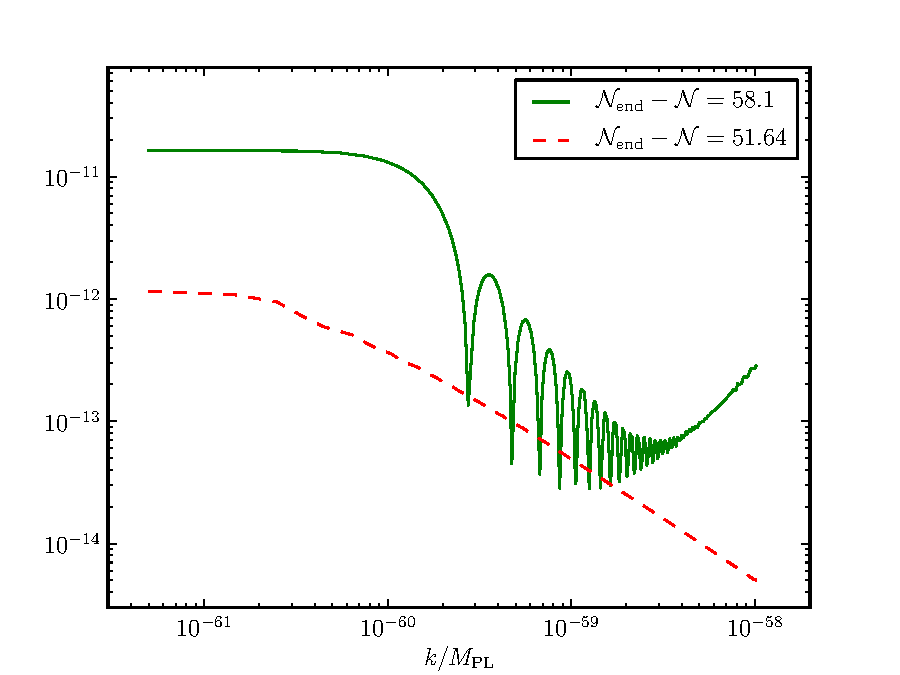
\includegraphics[width=0.8\textwidth]{numerical/graphs/src_3ns-large}
\caption[Source Term at Two Different Times]{The absolute magnitude of the source 
term for all $k$ values in the range $K_1$ at two different time steps. The green line shows
$|S|$ when all modes have been initialised. The lower red dashed line shows $|S|$ approximately 
52 e-foldings before the end of inflation, when all modes have
exited the horizon.}
\label{fig:src-3ns-2}
\end{figure}

\textbf{Each subfigure in Fig 8.11 has been changed to remove the erroneous sourceterm info before
the mode is initialised. The new figures are as shown in Fig~\ref{fig:newsrccmp}.
}

\begin{figure}[htbp]
\centering%
\subfloat[$V(\vp)=\msqphisq$]{
 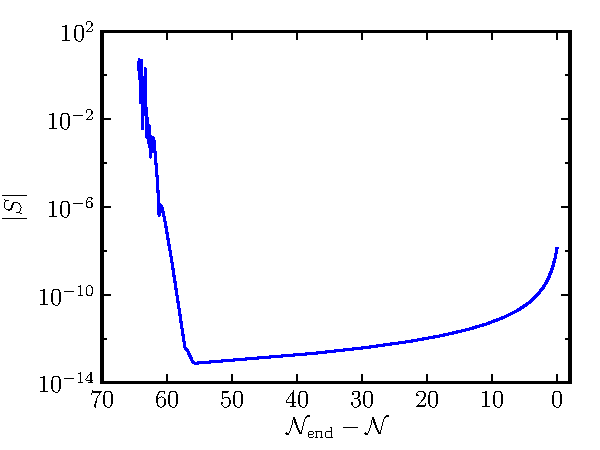
\includegraphics[width=0.43\textwidth]{numerical/graphs/src_onek_msqphisq-small}
}\qquad%
\subfloat[$V(\vp)=\lambdaphifour$]{
 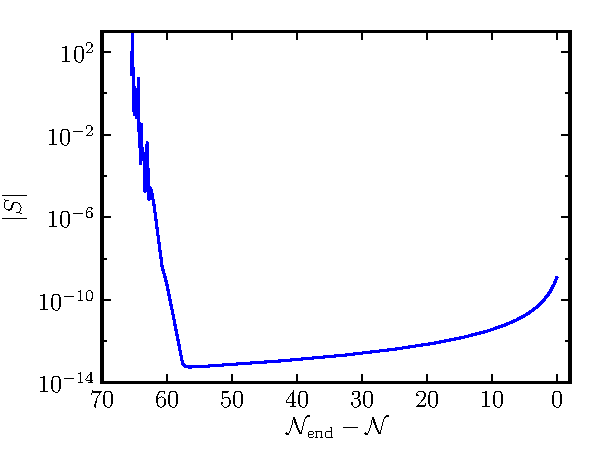
\includegraphics[width=0.43\textwidth]{numerical/graphs/src_onek_lambdaphi4-small}
}\\%
\subfloat[$V(\vp)=\phitwooverthree$]{
 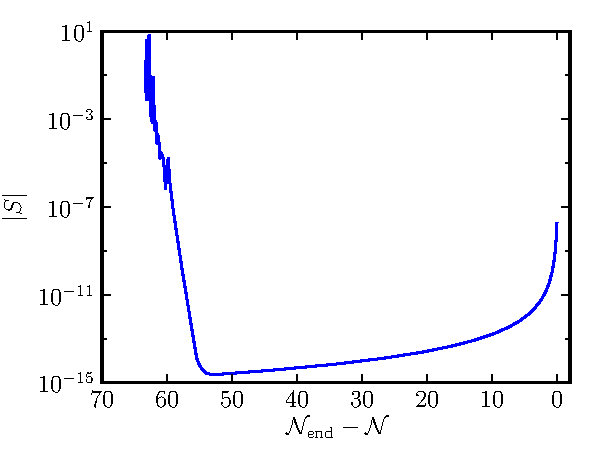
\includegraphics[width=0.43\textwidth]{numerical/graphs/src_onek_phi2over3-small}
}\qquad%
\subfloat[$V(\vp)=\msqphisqwithV$]{
 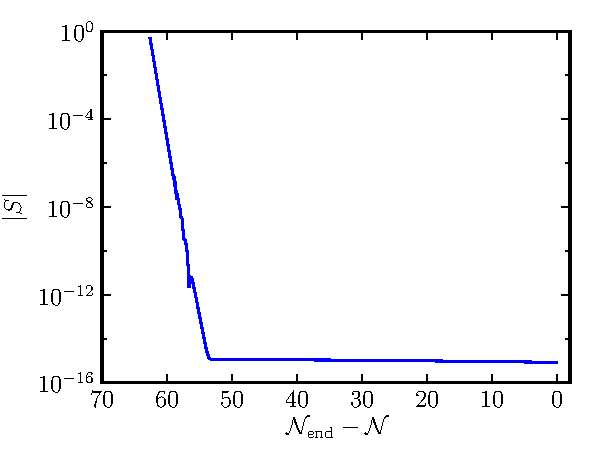
\includegraphics[width=0.43\textwidth]
  {numerical/graphs/src_onek_msqphisq_withV0-small}
}
\caption[Source Term for the Four Potentials]{Plots of the source
term for the
four different potentials studied.}
\label{fig:newsrccmp}
\end{figure}

\textbf{In the case of the other figures, especially Fig 8.4 on Pg 123 and Fig 8.5 on Pg 124, the
small oscillations at early times are not a numerical artifact. The first order perturbations at
these times are highly oscillatory as they have not yet been damped sufficiently. (See for example
Fig 8.1 on Pg 121.) In convolving the first order perturbations there is no expectation that
oscillations in one mode will be matched by those in another. At later times when the first order
modes are approximately constant the resulting source term is clearly smoother. 
}

\subsection{Point 15: Compare numerical results with analytic solution}

\textbf{Added as Section~\ref{sec:analytic-res} to Results Chapter:}
In this section results for the quadratic model will be compared with an analytic solution for this
model. However, an analytical result is difficult to obtain for the case of the full first
order solution in terms of Hankel functions with the phase information included. The analytical
solution we will use, therefore, is the non-interacting de Sitter
space solution with the phase information ignored. The first order perturbations are then given by
% 
\begin{equation}
 \dvp1(\eta, \kvi) = \frac{1}{a\sqrt{2 k}} \left( 1 - \frac{i}{k \eta}\right) \,,
\end{equation}
% 
and the derivative in terms of $\N$ is 
% 
\begin{equation}
 \dN{\dvp1}(\eta, \kvi) = -  \frac{1}{a\sqrt{2 k}} \left( 1 -
                        \frac{i}{k \eta}\right) \left(1 + \frac{1}{aH\eta}\right)
                         - \frac{i}{a^2 H \sqrt{2}}\sqrt{k}\,.
\end{equation}
% 

The source term is found using \eq{eq:KG2-source-ntime} and the values of the background
quantities. The analytical solution of \eq{eq:KG2-source-ntime} for this choice of first order
solution is given in Appendix~\ref{sec:analyticsrc-apx} in Eqs.
(\ref{eq:Jdefns-apx}-\ref{eq:JD-apx}).

In Figure~\ref{fig:analytic-61before-corr} the analytical and calculated solutions are plotted for
one timestep about 60 e-foldings before the end of inflation. At a single time step the correlation
between the two solutions for $S$ is very good. There is a deviation at small
values of $k$ due to the analytical solution getting rapidly smaller as $k$ approaches zero. This
 is not replicated in the calculated version. However, this only strongly affects the
result for the smallest values of $k$ and for $\kwmap$ for example the relative error of the
calculated solution compared to the analytical solution is about $10^{-4}$. The relative error of
the calculated solution is shown in Figure~\ref{fig:analytic-61before-errors-corr} for a single time
step.

\begin{figure}
 \centering
 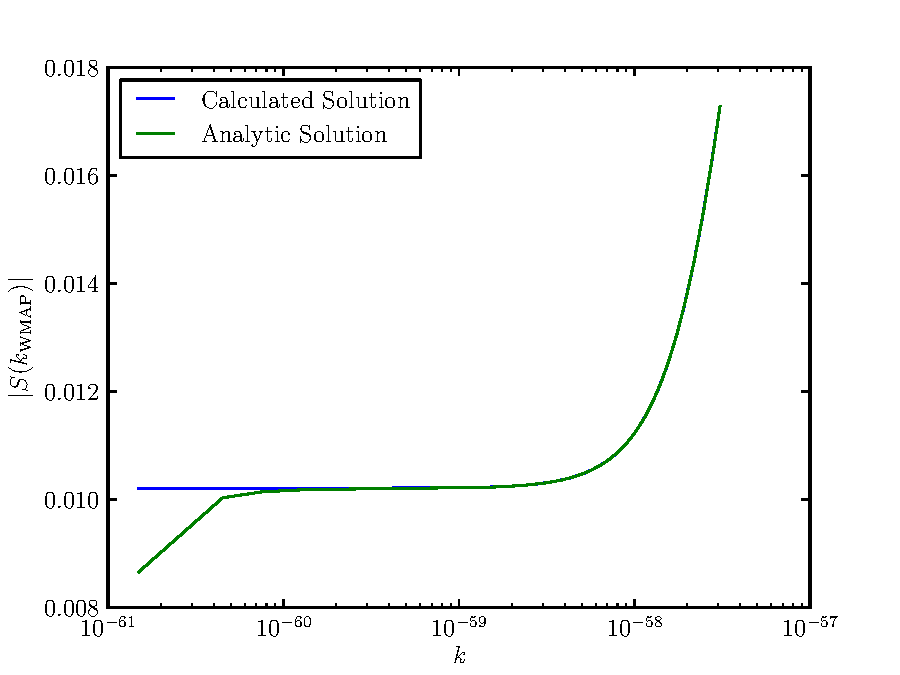
\includegraphics[width=0.8\textwidth]{numerical/graphs/analytic_v_calced_61beforeend-large}
 % analytic_v_calced_61beforeend-large.pdf: 432x324 pixel, 72dpi, 15.24x11.43 cm, bb=0 0 432 324
 \caption[Comparison of Analytical and Calculated Source Terms]{A comparison of the
analytical and calculated solutions for the source term at one time step, approximately 60
e-foldings before the end of inflation.}
 \label{fig:analytic-61before-corr}
\end{figure}

\begin{figure}
 \centering
 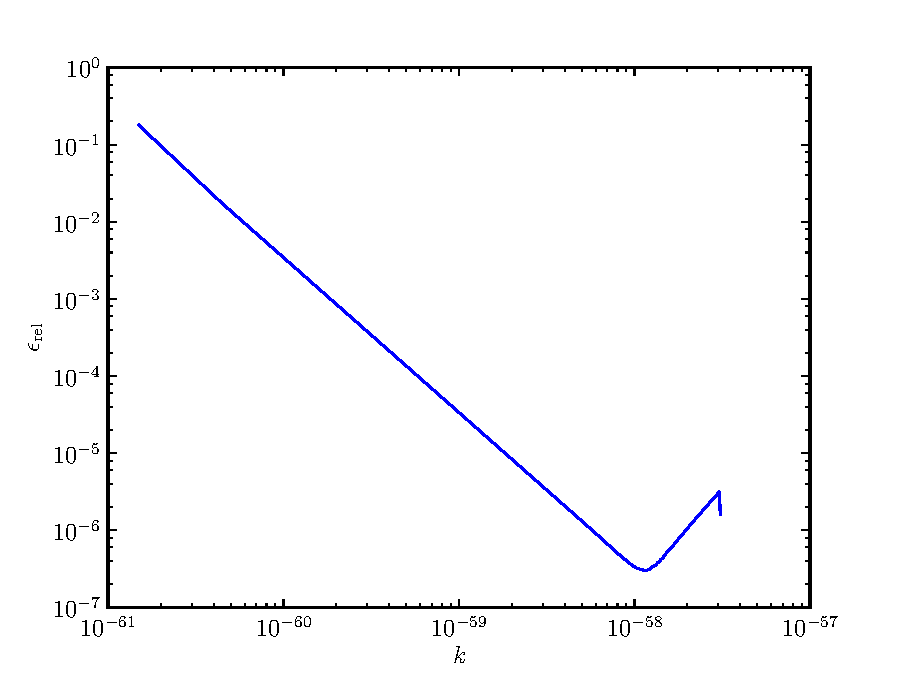
\includegraphics[width=0.8\textwidth]{numerical/graphs/analytic_v_calced_61beforeend_errors-large}
 \caption[Relative Error Of Calculated Solution at One Time Step]{The relative error of the
calculated solution compared to the analytical solution for the source term. The error is shown
for all $k$ values at one time step, approximately 60 e-foldings before the end of inflation.}
 \label{fig:analytic-61before-errors-corr}
\end{figure}

The analytical and calculated values for the source term can also be compared for a single $k$
value across a range of time steps. In Figure~\ref{fig:analytic-prehorizon-corr} the absolute
magnitude of the source term for $\kwmap$ is plotted for a range of a few e-foldings before horizon
crossing. The analytical and calculated results are extremely similar and not distinguishable in the
plot. The relative error of the calculated solution is around $10^{-4}$. Because the first order
perturbations do not include any phase information the result is much smoother than the result
generated using the full first order phase information. However, as the phase angle is a function of
$|\kvi-\qvi|$ it cannot be trivially ignored in the computation of the full convolution integral. 

\begin{figure}
 \centering
 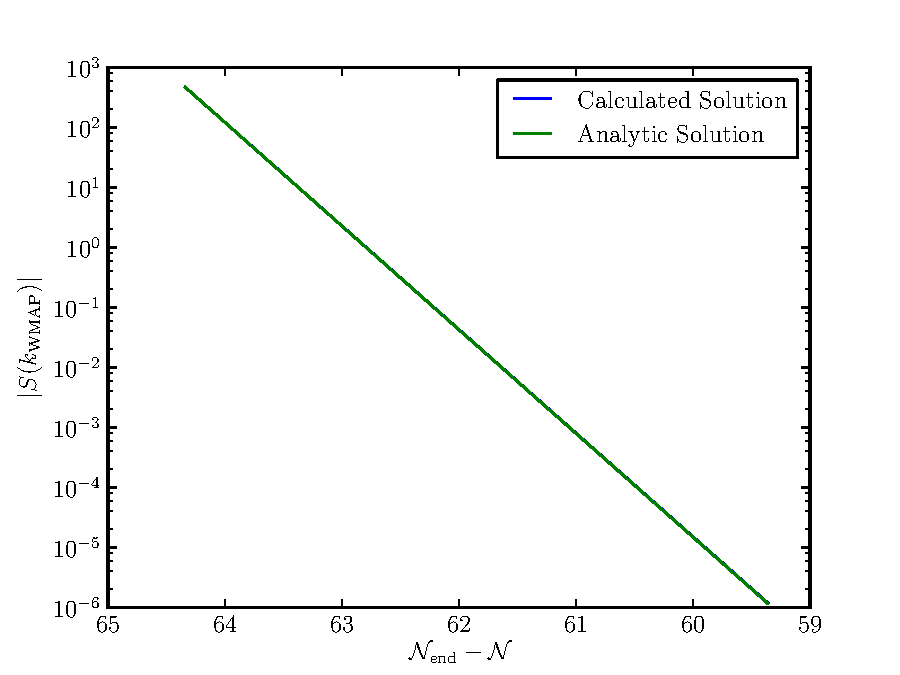
\includegraphics{numerical/graphs/analytic_v_calced_prehorizon-large.pdf}
 % analytic_v_calced_prehorizon-large.pdf: 432x324 pixel, 72dpi, 15.24x11.43 cm, bb=0 0 432 324
 \caption[Comparison of Solutions Before Horizon Crossing]{A comparison of the analytical and
calculated results for the source term of the $\kwmap$ mode before horizon crossing.}
 \label{fig:analytic-prehorizon-corr}
\end{figure}

\textbf{Added as Appendix~\ref{sec:analyticsrc-apx}:}

Suppose the first order perturbations are given by the non-interacting de Sitter space solution
such that
% 
 \begin{equation}
 \dvp1(\eta, \kvi) = \frac{1}{a\sqrt{2 k}} \left( 1 - \frac{i}{k \eta}\right) \,,
\end{equation}
% 
and the derivative in terms of $\N$ is 
% 
\begin{equation}
 \dN{\dvp1}(\eta, \kvi) = -  \frac{1}{a\sqrt{2 k}} \left( 1 -
                        \frac{i}{k \eta}\right) \left(1 + \frac{1}{aH\eta}\right)
                         - \frac{i}{a^2 H \sqrt{2}}\sqrt{k}\,.
\end{equation}
% 
The analytic solution of \eq{eq:KG2-source-ntime} for this choice of first order
solution can be written in terms of four integrals of the $\A$-$\wt{\D}$ terms:
% 
\begin{equation}
\label{eq:KG2-source-jterms-corr}
S(\kvi) = \frac{1}{(2\pi)^2} \left\{J_\A + J_\B + J_{\wt{\C}} + J_{\wt{\D}} \right\}\,,
\end{equation}
% 
where
\begin{align}
\label{eq:Jdefns-corr}
 J_\A(\kvi) &= \int_{\kmin}^{\kmax} \d q\, \left( 
                \frac{\Uppp}{H^2} q^2 + \frac{8\pi G}{(aH)^2}\dN{\vp_{0}}\left[ 
 3a^2\Upp q^2  + \frac{7}{2}q^4 + 2k^2q^2 \right] \right) \dvp1(\qvi) \A(\kvi, \qvi) \,, \\
% 
 J_\B(\kvi) &= \int_{\kmin}^{\kmax} \d q\, \frac{8\pi G}{(aH)^2}\dN{\vp_{0}}\left(-\frac{9}{2} -
\frac{q^2}{k^2}\right)kq^3 \dvp1(\qvi) \B(\kvi, \qvi) \,, \\
%  
J_{\wt{\C}}(\kvi) &= \int_{\kmin}^{\kmax} \d q\, \left(
                        -8\pi G \dN{\vp_{0}} \frac{3}{2}q^2 \right) \dN{\dvp1}(\qvi)
\wt{\C}(\kvi, \qvi) \,, \\
%  
J_{\wt{\D}}(\kvi) &= \int_{\kmin}^{\kmax} \d q\, \left(
                       8\pi G \dN{\vp_{0}} \left[2-\frac{q^2}{k^2}\right] kq \right)
\dN{\dvp1}(\qvi) \wt{\D}(\kvi, \qvi) \,. 
\end{align}
% 

The analytic solution for $J_\A$ is given by
\begin{multline}
\label{eq:JA-corr}
% 
J_\A = \left( 
                \frac{\Uppp}{H^2} + \frac{8\pi G}{(aH)^2}\dN{\vp_{0}}\left[ 
 3a^2\Upp    + 2k^2 \right] \right)\frac{ \alpha^2}{2880\eta ^2 k}\Bigg\{\\
240 k \arctan\left(\sqrt{\frac{\kmin}{k-\kmin}}\right) \left(\eta ^2 k^2-12 i \eta  k-24\right) \\
-120 k \pi  \left(\eta ^2 k^2-12 i \eta  k-24\right)
-80\sqrt{\kmax}
   \Bigg(\Bigg[3 \left(\sqrt{\kmax-k}-\sqrt{k+\kmax}\right) k^2 \\
-14 \kmax
   \left(\sqrt{\kmax-k}+\sqrt{k+\kmax}\right) k+8 \kmax^2
   \left(\sqrt{\kmax-k}-\sqrt{k+\kmax}\right)\Bigg] \eta ^2 \\
+48 i \left(\kmax
   \left(\sqrt{k+\kmax}-\sqrt{\kmax-k}\right)+k
   \left(\sqrt{\kmax-k}+\sqrt{k+\kmax}\right)\right) \eta \\
+72
   \left(\sqrt{k+\kmax}-\sqrt{\kmax-k}\right)\Bigg) \displaybreak[0]\\
% 
-80 \sqrt{\kmin} \Bigg(\Bigg[3
   \left(\sqrt{k-\kmin}+\sqrt{k+\kmin}\right) k^2
-14 \kmin\left(\sqrt{k-\kmin}-\sqrt{k+\kmin}\right) k \\
+8 \kmin^2
   \left(\sqrt{k-\kmin}+\sqrt{k+\kmin}\right)\Bigg] \eta ^2
+12 i \Bigg[k
   \left(\sqrt{k-\kmin}-4 \sqrt{k+\kmin}\right) \\
+2 \kmin
\left(\sqrt{k-\kmin}-2
   \sqrt{k+\kmin}\right)\Bigg] \eta +72
   \left(\sqrt{k-\kmin}-\sqrt{k+\kmin}\right)\Bigg) \displaybreak[0]\\
% 
+240 k \left(\eta ^2 k^2+24\right)\log\left(2 \sqrt{k}\right)
-240 k \left(\eta ^2 k^2+24\right)\log \left(2 \left(\sqrt{\kmax}+\sqrt{\kmax-k}\right)\right)\\
-240 k \left(\eta ^2 k^2+24\right) \log \left(2\left(\sqrt{\kmax}+\sqrt{k+\kmax}\right)\right)\\
+240 k \left(\eta ^2 k^2+24\right) \log
\left(2 \left(\sqrt{\kmin}+\sqrt{k+\kmin}\right)\right)\Bigg\} \displaybreak[0]\\
% 
%
+ \frac{8\pi G}{(aH)^2}\dN{\vp_{0}}\frac{7}{2}\frac{\alpha ^2}{2880 \eta
^2 k} \Bigg\{3 \sqrt{2} \left(-317 \eta ^2 k^2+1000 i \eta  k+560\right) k^3 \\
+3\sqrt{2} \left(317 \eta ^2 k^2-1000 i \eta  k-560\right) k^3 \\
+45 \left(\eta ^2 k^2-12 i \eta k-16\right) \arctan\left(\sqrt{\frac{\kmin}{k-\kmin}}\right) k^3
+45\left(\eta ^2 k^2+8 i \eta k+16\right)
   \log \left(2 \sqrt{k}\right) k^3 \\
-45 \left(\eta ^2 k^2+8 i \eta  k+16\right) \log \left(2
   \left(\sqrt{\kmax}+\sqrt{\kmax-k}\right)\right) k^3 \\
-45 \left(\eta ^2 k^2-8 i \eta 
   k+16\right) \log \left(2 \left(\sqrt{\kmax}+\sqrt{k+\kmax}\right)\right) k^3 \\
+45\left(\eta ^2 k^2-8 i \eta  k+16\right) \log \left(2
\left(\sqrt{\kmin}+\sqrt{k+\kmin}\right)\right) k^3 -\frac{45}{2} \left(\eta ^2 k^2-12 i \eta 
k-16\right) \pi  k^3 \displaybreak[0]\\
% 
-3 \sqrt{\kmax} \Bigg(15 \eta ^2
   \left(\sqrt{\kmax-k}-\sqrt{k+\kmax}\right) k^4 \\
 +10 \eta  (\eta  \kmax+12 i)
   \left(\sqrt{\kmax-k}+\sqrt{k+\kmax}\right) k^3 \\ 
+8 \left(\eta ^2 \kmax^2+10 i \eta 
   \kmax+30\right) \left(\sqrt{\kmax-k}-\sqrt{k+\kmax}\right) k^2 \\
-16 \kmax \left(11\eta ^2 \kmax^2-20 i \eta  \kmax-10\right)
   \left(\sqrt{\kmax-k}+\sqrt{k+\kmax}\right) k \\
+128 \kmax^2 \left(\eta ^2 \kmax^2-5i \eta  \kmax-5\right)
\left(\sqrt{\kmax-k}-\sqrt{k+\kmax}\right)\Bigg) \displaybreak[0]\\
%  
-3 \sqrt{\kmin} \Bigg(15 \eta ^2 \left(\sqrt{k-\kmin}+\sqrt{k+\kmin}\right) k^4 \\
+10 \eta\left(\eta  \kmin \left(\sqrt{k-\kmin}-\sqrt{k+\kmin}\right)-6 i \left(3
   \sqrt{k-\kmin}+2 \sqrt{k+\kmin}\right)\right) k^3 \\
+8 \Bigg(\eta ^2
   \left(\sqrt{k-\kmin}+\sqrt{k+\kmin}\right) \kmin^2-5 i \eta  \left(3
   \sqrt{k-\kmin}-2 \sqrt{k+\kmin}\right) \kmin \\
+30
   \left(\sqrt{k+\kmin}-\sqrt{k-\kmin}\right)\Bigg) k^2 \displaybreak[0]\\
-16 \kmin \Bigg(11 \eta ^2
   \left(\sqrt{k-\kmin}-\sqrt{k+\kmin}\right) \kmin^2-10 i \eta 
   \left(\sqrt{k-\kmin}-2 \sqrt{k+\kmin}\right) \kmin \\+10
   \left(\sqrt{k-\kmin}+\sqrt{k+\kmin}\right)\Bigg) k \\
+64 \kmin^2 \Bigg(2 \eta ^2
   \left(\sqrt{k-\kmin}+\sqrt{k+\kmin}\right) \kmin^2+5 i \eta 
   \left(\sqrt{k-\kmin}-2 \sqrt{k+\kmin}\right) \kmin \\
+10
   \left(\sqrt{k-\kmin}-\sqrt{k+\kmin}\right)\Bigg)\Bigg)\Bigg\}\,. 
\end{multline}

The analytic solution for $J_\B$ is 
% 
\begin{multline}
\label{eq:JB-corr}
% 
J_\B = -\frac{8\pi G}{(aH)^2}\dN{\vp_{0}}\frac{9}{2}\frac{\alpha ^2}{2822400 \eta ^2
k} \Bigg\{29400 \left(4 \eta ^2 k^2+15 i \eta k+120\right)
\arctan\left(\sqrt{\frac{\kmin}{k-\kmin}}\right) k^3 \\
+29400 \left(4 \eta ^2 k^2-51 i \eta 
   k-120\right) \log \left(2 \sqrt{k}\right) k^3 \\
-29400 \left(4 \eta ^2 k^2-51 i \eta k-120\right) \log
   \left(2 \left(\sqrt{\kmax}+\sqrt{\kmax-k}\right)\right) k^3 \\
-29400 \left(4 \eta ^2 k^2+51 i \eta  k-120\right) \log \left(2
\left(\sqrt{\kmax}+\sqrt{k+\kmax}\right)\right) k^3 \\
+29400 \left(4 \eta ^2 k^2+51 i \eta  k-120\right) \log \left(2
   \left(\sqrt{\kmin}+\sqrt{k+\kmin}\right)\right) k^3 \\
-14700 \left(4 \eta ^2 k^2+15 i
\eta 
   k+120\right) \pi  k^3 
+280 \sqrt{\kmax (k+\kmax)} \Bigg(420 \eta ^2 k^4 \\
+5 \eta  (200 \eta \kmax+303 i) k^3 + \left(-416 \eta ^2 \kmax^2+6414 i \eta  \kmax+11592\right)
k^2 \\ 
- 24\kmax \left(8 \eta ^2 \kmax^2-87 i \eta  \kmax-126\right) k 
+48 \kmax^2\left(8\eta ^2 \kmax^2+53 i \eta  \kmax+84\right)\Bigg) \displaybreak[0]\\
% 
-280 \sqrt{\kmax (\kmax-k)}
   \Bigg(420 \eta ^2 k^4-5 \eta  (200 \eta  \kmax+303 i) k^3 \\
+\left(-416 \eta ^2 \kmax^2+6414 i
   \eta  \kmax+11592\right) k^2+24 \kmax \left(8 \eta ^2 \kmax^2-87 i \eta 
   \kmax-126\right) k \\
+48 \kmax^2 \left(8 \eta ^2 \kmax^2+53 i \eta 
   \kmax+84\right)\Bigg) \displaybreak[0] \\
% 
-280 \sqrt{\kmin} \sqrt{k+\kmin} \Bigg(420 \eta ^2 k^4+5
\eta 
   (200 \eta  \kmin+303 i) k^3 \\
+\left(-416 \eta ^2 \kmin^2+6414 i \eta \kmin+11592\right)k^2 -24 \kmin \left(8 \eta ^2 \kmin^2-87
i \eta  \kmin-126\right) k \\
+48 \kmin^2 \left(8 \eta ^2 \kmin^2+53 i \eta  \kmin+84\right)\Bigg) \displaybreak[0]\\
-280 \sqrt{(k-\kmin)
   \kmin} \Bigg(420 \eta ^2 k^4+5 \eta  (1083 i-200 \eta  \kmin) k^3 \\
-2 \left(208 \eta ^2
   \kmin^2+2547 i \eta  \kmin+5796\right) k^2+24 \kmin \left(8 \eta ^2
\kmin^2+67 i
   \eta  \kmin+126\right) k \\
+48 \kmin^2 \left(8 \eta ^2 \kmin^2-73 i \eta 
   \kmin-84\right)\Bigg)\Bigg\} \displaybreak[1]\\
% 
% 
- \frac{8\pi G}{(aH)^2}\dN{\vp_{0}}\frac{\alpha ^2}{2822400 \eta ^2 k^3} \Bigg\{105
\left(270 \eta ^2 k^2+2765 i \eta  k+4956\right) \arctan \left(\sqrt{\frac{\kmin}{k-\kmin}}\right)
   k^5 \\
+105 \left(270 \eta ^2 k^2-3745 i \eta  k-4956\right) \log \left(2 \sqrt{k}\right) k^5\\
-105\left(270 \eta ^2 k^2-3745 i \eta  k-4956\right) \log \left(2
   \left(\sqrt{\kmax}+\sqrt{\kmax-k}\right)\right) k^5 \\
-105 \left(270 \eta ^2 k^2+3745 i \eta 
   k-4956\right) \log \left(2 \left(\sqrt{\kmax}+\sqrt{k+\kmax}\right)\right) k^5 \\
+105\left(270  \eta ^2 k^2+3745 i \eta  k-4956\right) \log \left(2
   \left(\sqrt{\kmin}+\sqrt{k+\kmin}\right)\right) k^5 \\
-\frac{105}{2} \left(270 \eta ^2 k^2+2765 i \eta  k+4956\right) \pi  k^5\displaybreak[0]\\
% 
-\sqrt{\kmax (\kmax-k)} \Bigg(28350 \eta ^2 k^6+525 \eta  (36
   \eta  \kmax-749 i) k^5 \\
+70 \left(216 \eta ^2 \kmax^2-3745 i \eta\kmax-7434\right) k^4 
-40 \kmax \left(3516 \eta ^2 \kmax^2-133 i \eta  \kmax+8673\right) k^3 \\
-48 \kmax^2 \left(1360 \eta ^2 \kmax^2-18655 i \eta  \kmax-22442\right) k^2 \\
+64 \kmax^3 \left(600 \eta ^2 \kmax^2-5110 i \eta  \kmax-5733\right) k \\
+256\kmax^4 \left(300 \eta ^2 \kmax^2+1855 i \eta  \kmax+2646\right)\Bigg) \displaybreak[0]\\
% 
+\sqrt{\kmax(k+\kmax)} \Bigg(28350 \eta ^2 k^6-525 \eta  (36 \eta  \kmax-749 i) k^5 \\
+70 \left(216 \eta ^2  \kmax^2-3745 i \eta  \kmax-7434\right) k^4
+40 \kmax \left(3516 \eta ^2 \kmax^2-133 i \eta  \kmax+8673\right) k^3 \\
-48 \kmax^2 \left(1360 \eta^2 \kmax^2-18655 i \eta  \kmax-22442\right) k^2
-64 \kmax^3 \left(600\eta ^2 \kmax^2-5110 i \eta  \kmax-5733\right) k \\
+256 \kmax^4 \left(300 \eta^2 \kmax^2+1855 i \eta  \kmax+2646\right)\Bigg) \displaybreak[0] \\
% 
-\sqrt{\kmin} \sqrt{k+\kmin}
   \Bigg(28350 \eta ^2 k^6-525 \eta  (36 \eta  \kmin-749 i) k^5 \\
+70 \left(216 \eta ^2 \kmin^2-3745 i \eta  \kmin-7434\right) k^4
+40 \kmin \left(3516 \eta ^2 \kmin^2-133 i \eta  \kmin+8673\right) k^3 \\
-48 \kmin^2 \left(1360 \eta^2 \kmin^2-18655 i \eta  \kmin-22442\right) k^2
-64 \kmin^3 \left(600\eta ^2 \kmin^2-5110 i \eta  \kmin-5733\right) k \\
+256 \kmin^4 \left(300 \eta^2\kmin^2+1855 i \eta  \kmin+2646\right)\Bigg) \displaybreak[0]\\
-\sqrt{(k-\kmin) \kmin}\Bigg(28350 \eta ^2 k^6+525 \eta  (36 \eta  \kmin+553 i) k^5 \\
+70 \left(216\eta ^2 \kmin^2+2765 i \eta\kmin+7434\right) k^4 
-40 \kmin \left(3516 \eta ^2\kmin^2-9247 i \eta\kmin-8673\right) k^3 \\
-48 \kmin^2 \left(1360 \eta^2 \kmin^2+15155 i \eta\kmin+22442\right) k^2 
+64 \kmin^3 \left(600\eta ^2 \kmin^2+3710 i \eta\kmin+5733\right) k \\
+256 \kmin^4 \left(300 \eta ^2\kmin^2-2555 i \eta\kmin-2646\right)\Bigg)\Bigg\}\,.
\end{multline}

The analytic solution for $J_{\wt{\C}}$ is 
% 
\begin{multline}
\label{eq:JC-corr}
% 
 J_{\wt{\C}} = -8\pi G \dN{\vp_{0}} \frac{3}{2} \frac{\alpha ^2 }{14400 \beta ^2 \eta ^4 k}
\Bigg\{-15 k \arctan\left(\sqrt{\frac{\kmin}{k-\kmin}}\right)
   \Bigg(9 \eta ^4 k^4-60 i \eta ^3 k^3-560 \eta ^2 k^2 \\
+960 i \eta  k-80 \beta ^2 \eta ^2 \left(\eta ^2 k^2-12 i \eta  k-24\right) 
+20 \beta  \eta\left(-3 i \eta ^3 k^3-32 \eta ^2 k^2+96 i \eta k+192\right)+1920\Bigg)
\displaybreak[0]\\
% 
+\frac{15}{2} k \pi  \Bigg(9 \eta ^4 k^4-60 i \eta ^3 k^3-560 \eta ^2
k^2+960 i
   \eta  k-80 \beta ^2 \eta ^2 \left(\eta ^2 k^2-12 i \eta  k-24\right) \\
+20 \beta  \eta  \left(-3 i\eta ^3 k^3-32 \eta ^2 k^2+96 i \eta  k+192\right)+1920\Bigg)
\displaybreak[0]\\
% 
-\sqrt{\kmax (\kmax-k)} \Bigg(9 \left(15 k^4+10 \kmax k^3-248 \kmax^2 k^2+336 \kmax^3 k
-128\kmax^4\right) \eta ^4 \\
+3840 i (k-\kmax)^2 \kmax \eta ^3 +80 \left(69 k^2-178 \kmax k+184 \kmax^2\right) \eta ^2 \\ 
+400 \beta ^2 \left(\left(3 k^2-14 \kmax k+8 \kmax^2\right) \eta^2 
+48 i (k-\kmax) \eta -72\right)\eta ^2+19200 i (k-\kmax) \eta \\
+320 \beta  \Bigg[12 i   (k-\kmax)^2 \kmax \eta ^3+\left(21 k^2-62 \kmax k+56 \kmax^2\right) \eta
^2 \\
+120 i(k-\kmax) \eta  -180\Bigg] \eta -28800\Bigg) \displaybreak[0] \\
% 
+\sqrt{\kmax (k+\kmax)} \Bigg(9\left(15 k^4-10 \kmax k^3-248 \kmax^2 k^2-336 \kmax^3 k-128
\kmax^4\right) \eta ^4 \\
+3840 i \kmax (k+\kmax)^2 \eta ^3+80 \left(69 k^2+178 \kmax k+184 \kmax^2\right)\eta^2 \\
+400 \beta^2 \left(\left(3 k^2+14 \kmax k+8 \kmax^2\right) \eta ^2 -48 i (k+\kmax)
   \eta -72\right) \eta ^2 \\
-19200 i (k+\kmax) \eta +320 \beta  \Bigg[12 i \kmax
(k+\kmax)^2 \eta ^3+\left(21 k^2+62 \kmax k+56 \kmax^2\right) \eta ^2 \\
-120 i (k+\kmax) \eta -180\Bigg] \eta -28800\Bigg) \displaybreak[0] \\
% 
+\sqrt{\kmin} \sqrt{k+\kmin} \Bigg(9 \left(-15 k^4+10  \kmin k^3+248 \kmin^2 k^2+336 \kmin^3 k+128
\kmin^4\right) \eta ^4 \\
-3840 i \kmin (k+\kmin)^2 \eta ^3-80 \left(69 k^2+178 \kmin k+184 \kmin^2\right)\eta^2 \\
-400 \beta ^2 \left(\left(3 k^2+14 \kmin k+8 \kmin^2\right) \eta ^2-48 i(k+\kmin)
   \eta -72\right) \eta ^2 \\
+19200 i (k+\kmin) \eta +320 \beta  \Bigg[-12 i \kmin
   (k+\kmin)^2 \eta ^3-\left(21 k^2+62 \kmin k+56 \kmin^2\right) \eta ^2 \\
+120 i(k+\kmin) \eta +180\Bigg] \eta +28800\Bigg) \displaybreak[0]\\
% 
-\sqrt{(k-\kmin) \kmin} \Bigg(-9\left(15
   k^4+10 \kmin k^3-248 \kmin^2 k^2+336 \kmin^3 k-128 \kmin^4\right) \eta^4 \\
+60 i \left(15 k^3-54 \kmin k^2+8 \kmin^2 k+16 \kmin^3\right) \eta ^3
-80 \left(39k^2-38  \kmin k+104 \kmin^2\right) \eta ^2 \\
+400 \beta ^2 \left(\left(3 k^2-14 \kmin k+8 \kmin^2\right) \eta ^2+12 i (k+2 \kmin) \eta
+72\right) \eta ^2 \\
+4800 i (k+2 \kmin) \eta +20 i \beta  \Bigg[3 \left(15 k^3-54 \kmin k^2+8 \kmin^2 k+16
\kmin^3\right) \eta ^3 \\
+32 i \left(3 k^2+4 \kmin k+8 \kmin^2\right) \eta ^2+480 (k+2 \kmin) \eta -2880
i\Bigg]
   \eta +28800\Bigg) \displaybreak[0] \\
% 
+15 k \left(9 \eta ^4 k^4-400 \eta ^2 k^2-320 \beta  \eta 
\left(\eta ^2
   k^2-12\right)+80 \beta ^2 \eta ^2 \left(\eta ^2 k^2+24\right)+1920\right) \log \left(2
\sqrt{k}\right) \\
-15k \Bigg(9 \eta ^4 k^4-400 \eta ^2 k^2-320 \beta  \eta  \left(\eta ^2 k^2-12\right)\\
+80 \beta ^2\eta ^2 \left(\eta ^2 k^2+24\right)+1920\Bigg) \log \left(2
   \left(\sqrt{\kmax}+\sqrt{\kmax-k}\right)\right) \\
-15 k \Bigg(9 \eta ^4 k^4-400 \eta ^2 k^2-320
   \beta  \eta  \left(\eta ^2 k^2-12\right) \\
+80 \beta ^2 \eta ^2 \left(\eta ^2
k^2+24\right)+1920\Bigg) \log \left(2 \left(\sqrt{\kmax}+\sqrt{k+\kmax}\right)\right) \\
+15 k \Bigg(9 \eta ^4 k^4-400\eta ^2 k^2-320 \beta  \eta  \left(\eta ^2 k^2-12\right) \\
+80 \beta ^2 \eta ^2 \left(\eta ^2 k^2+24\right)+1920\Bigg) \log \left(2
   \left(\sqrt{\kmin}+\sqrt{k+\kmin}\right)\right)\Bigg\} \,.
\end{multline}

The analytic solution for $J_{\wt{\D}}$ is 
% 
\begin{multline}
\label{eq:JD-corr}
% 
J_{\wt{\D}} = 8\pi G \dN{\vp_{0}}\frac{\alpha ^2}{302400\beta ^2\eta ^4 k} 
\Bigg\{-5040 k \arctan\left(\sqrt{\frac{\kmin}{k-\kmin}}\right) \Bigg(9 \eta ^4 k^4 
+230 \eta ^2 k^2+260 i \eta k\\
+20 \beta ^2 \eta ^2 \left(2 \eta ^2 k^2+13 i \eta  k-12\right) 
+10\beta \eta \left(27 \eta^2 k^2+52 i \eta  k-48\right)-240\Bigg) \displaybreak[0]\\
+2520 k \pi\Bigg(9 \eta ^4 k^4+230 \eta ^2 k^2+260 i \eta  k+20
\beta ^2\eta ^2 \left(2 \eta ^2 k^2+13 i \eta  k-12\right)\\
+10 \beta  \eta  \left(27 \eta ^2 k^2+52 i\eta k-48\right)-240\Bigg)
+\frac{16\sqrt{k+\kmax}}{\kmax^{3/2}} \Bigg(-35 \eta ^2 \Bigg(111 \eta ^2
   \kmax^2 \displaybreak[0]\\
+192 i \eta  \kmax+64 \beta  \eta  (3 i \eta  \kmax+1)+64\Bigg) k^4
-5\eta\Bigg(-294 \eta ^3 \kmax^3-717 i \eta ^2 \kmax^2+2656 \eta  \kmax \\
+960 \beta ^2\eta ^2 (3 \eta  \kmax-i)+\beta  \eta  \left(-717 i \eta ^2 \kmax^2+5536 \eta 
\kmax-1920 i\right)-960 i\Bigg) k^3 \\
-6 \Bigg(-588 \eta ^4 \kmax^4+1305 i \eta ^3 \kmax^3+9965
\eta ^2 \kmax^2+15520 i \eta  \kmax\displaybreak[0]\\
+20 \beta ^2 \eta ^2 \left(45 \eta ^2\kmax^2+776 i\eta\kmax+252\right)+5 \beta\eta\Bigg(261 i
\eta ^3 \kmax^3+2173 \eta ^2\kmax^2 
+6208 i\eta  \kmax+2016\Bigg) \displaybreak[0]\\
+5040\Bigg) k^2 +4 \kmax \Bigg(84 \eta ^4 \kmax^4-330 i\eta ^3 \kmax^3-3275 \eta ^2 \kmax^2+7065 i
\eta  \kmax-15 \beta ^2 \eta ^2 \Bigg(20\eta ^2 \kmax^2 \\
-471 i \eta  \kmax+1008\Bigg)-5 \beta\eta  \left(66 i \eta ^3\kmax^3+715\eta ^2 \kmax^2-2826 i \eta 
\kmax+6048\right)-15120\Bigg) k\\
+8 \kmax^2\Bigg(-84 \eta^4 \kmax^4+330 i \eta ^3 \kmax^3-1450 \eta ^2 \kmax^2+2385 i \eta 
\kmax+15 \beta^2 \eta ^2 \Bigg(20 \eta ^2 \kmax^2\\
+159 i \eta  \kmax+378\Bigg)+10 \beta  \eta\left(33 i \eta ^3 \kmax^3-115 \eta ^2 \kmax^2+477 i
\eta \kmax+1134\right)+5670\Bigg)\Bigg)\displaybreak[0]\\
+16\kmax^{-3/2} \sqrt{\kmax-k}\Bigg(35\eta ^2 \left(111 \eta ^2 \kmax^2+192 i \eta 
\kmax+64 \beta \eta  (3 i \eta \kmax+1)+64\right) k^4\\
+5 \eta  \Bigg(294 \eta ^3 \kmax^3+717 i \eta^2 \kmax^2-2656
   \eta  \kmax-960 \beta ^2 \eta ^2 (3 \eta  \kmax-i) \\
+i \beta  \eta  \left(717 \eta ^2  \kmax^2+5536 i \eta  \kmax+1920\right)+960 i\Bigg) k^3+6
\Bigg(-588 \eta ^4\kmax^4+1305 i \eta ^3 \kmax^3 \\
+9965 \eta ^2 \kmax^2+15520 i \eta\kmax+20 \beta
   ^2 \eta ^2 \left(45 \eta ^2 \kmax^2+776 i \eta  \kmax+252\right) \\
+5 \beta  \eta\left(261 i \eta ^3 \kmax^3+2173 \eta ^2 \kmax^2+6208 i \eta 
\kmax+2016\right)+5040\Bigg)k^2
+4 \kmax \Bigg(84 \eta ^4 \kmax^4 \\
-330 i \eta ^3 \kmax^3-3275 \eta ^2\kmax^2+7065 i\eta  \kmax-15 \beta ^2 \eta ^2 \left(20 \eta ^2
\kmax^2-471 i \eta \kmax+1008\right)\\
-5 \beta  \eta  \left(66 i \eta ^3 \kmax^3+715 \eta ^2\kmax^2-2826 i
   \eta  \kmax+6048\right)-15120\Bigg) k \displaybreak[0] \\
-8 \kmax^2 \Bigg(-84 \eta ^4 \kmax^4+330i \eta^3 \kmax^3-1450 \eta ^2 \kmax^2+2385 i \eta 
\kmax+15 \beta ^2 \eta ^2 \bigg(20\eta ^2 \kmax^2\\
+159 i \eta  \kmax+378\bigg)+10 \beta  \eta\left(33 i \eta ^3\kmax^3-115 \eta ^2 \kmax^2+477 i \eta 
\kmax+1134\right)+5670\Bigg)\Bigg)\displaybreak[0]\\
% 
+16 \kmin^{-3/2}
   \sqrt{k+\kmin} \Bigg(35 \eta ^2 \left(111 \eta ^2 \kmin^2+192 i \eta  \kmin+64
\beta \eta  (3 i \eta  \kmin+1)+64\right) k^4 \\
-5 \eta  \Bigg(294 \eta ^3 \kmin^3+717 i \eta^2\kmin^2-2656 \eta  \kmin-960 \beta ^2 \eta ^2 (3
\eta  \kmin-i) \\
+i \beta  \eta\left(717 \eta ^2 \kmin^2+5536 i \eta  \kmin+1920\right)+960 i\Bigg) k^3
+6\Bigg(-588 \eta ^4 \kmin^4 \\
+1305 i \eta ^3 \kmin^3+9965 \eta ^2 \kmin^2+15520 i \eta 
\kmin+20 \beta ^2 \eta ^2 \left(45 \eta ^2 \kmin^2+776 i \eta  \kmin+252\right) \\
+5 \beta  \eta \left(261 i \eta ^3 \kmin^3+2173 \eta ^2 \kmin^2+6208 i \eta 
   \kmin+2016\right)+5040\Bigg) k^2\displaybreak[0]\\
-4 \kmin \Bigg(84 \eta ^4 \kmin^4-330 i \eta^3\kmin^3-3275 \eta ^2 \kmin^2+7065 i \eta  \kmin-15
\beta ^2 \eta ^2 \bigg(20\eta ^2\kmin^2\\
-471 i \eta  \kmin+1008\bigg)
-5 \beta  \eta  \left(66 i\eta ^3\kmin^3+715 \eta ^2 \kmin^2-2826 i \eta 
\kmin+6048\right)-15120\Bigg) k\\
-8 \kmin^2\Bigg(-84 \eta^4 \kmin^4+330 i \eta ^3 \kmin^3-1450 \eta ^2 \kmin^2+2385 i \eta 
\kmin+15 \beta^2 \eta ^2 \bigg(20 \eta ^2 \kmin^2 \\
+159 i \eta  \kmin+378\bigg)+10 \beta  \eta\left(33 i
   \eta ^3 \kmin^3-115 \eta ^2 \kmin^2+477 i \eta 
   \kmin+1134\right)+5670\Bigg)\Bigg)\displaybreak[0]\\
% 
-16\kmin^{-3/2}\sqrt{k-\kmin}\Bigg(35\eta ^2 \left(111 \eta ^2 \kmin^2+192 i \eta  \kmin+64 \beta
 \eta  (3 i \eta \kmin+1)+64\right) k^4\\
+10 \eta  \Bigg(147 \eta ^3 \kmin^3-1104 i \eta ^2\kmin^2+1552
   \eta  \kmin+480 \beta ^2 \eta ^2 (3 \eta  \kmin-i)\\
+16 \beta  \eta  \left(-69 i \eta^2  
\kmin^2+187 \eta  \kmin-60 i\right)-480 i\Bigg) k^3+6 \Bigg(-588 \eta ^4
\kmin^4+480 i\eta ^3 \kmin^3\\
+8165 \eta ^2 \kmin^2+14720 i \eta  \kmin-20 \beta ^2 \eta ^2\left(45
   \eta ^2 \kmin^2-736 i \eta  \kmin-252\right)\\
+5 \beta  \eta  \left(96 i \eta ^3 \kmin^3+1453 \eta ^2 \kmin^2+5888 i \eta 
\kmin+2016\right)+5040\Bigg) k^2 \\
+4 \kmin \Bigg(84 \eta ^4 \kmin^4+120 i \eta ^3 \kmin^3-2675 \eta ^2\kmin^2+6165 i\eta  \kmin+15
\beta ^2 \eta ^2 \bigg(20 \eta ^2 \kmin^2 \\
+411 i \eta\kmin-1008\bigg)+5 i \beta  \eta  \left(24 \eta ^3 \kmin^3+475 i \eta ^2
\kmin^2+2466 \eta  \kmin+6048 i\right)-15120\Bigg) k\displaybreak[0]\\
+8 \kmin^2 \bigg(84 \eta ^4\kmin^4+120i \eta^3 \kmin^3+2050 \eta ^2 \kmin^2-3285 i \eta  \kmin+15
\beta ^2 \eta ^2 \bigg(20\eta ^2\kmin^2 \\
-219 i \eta  \kmin-378\bigg)+10 \beta  \eta  \left(12 i
\eta ^3\kmin^3+235  \eta ^2 \kmin^2-657 i \eta 
\kmin-1134\right)-5670\bigg)\Bigg) \displaybreak[0]\\
% 
-5040 k\bigg(-9 \eta ^4 k^4-45 i \eta ^3 k^3-150 \eta ^2 k^2-340 i \eta  k+20 \beta ^2 \eta ^2
\left(2\eta ^2 k^2-17 i \eta  k+12\right)\\
+5 \beta  \eta  \left(-9 i \eta ^3 k^3-22 \eta ^2 k^2-136
i \eta k+96\right)+240\bigg) \log \left(2 \sqrt{k}\right)\\
+5040 k \bigg(-9 \eta ^4 k^4-45 i \eta^3 k^3-150 \eta^2 k^2-340 i \eta  k+20 \beta ^2 \eta ^2
\left(2 \eta ^2 k^2-17 i \eta  k+12\right)\\
+5 \beta \eta \left(-9 i \eta ^3 k^3-22 \eta ^2 k^2-136 i \eta  k+96\right)+240\bigg) \log
\left(2 \left(\sqrt{\kmax}+\sqrt{\kmax-k}\right)\right) \\
+5040 k \bigg(-9 \eta ^4 k^4+45 i \eta^3 k^3-150 \eta ^2 k^2+340 i \eta  k+20 \beta ^2 \eta ^2
\left(2 \eta ^2 k^2+17 i \eta k+12\right)\\
+5 \beta\eta  \left(9 i \eta ^3 k^3-22 \eta ^2 k^2+136 i \eta  k+96\right)+240\bigg) \log \left(2
   \left(\sqrt{\kmax}+\sqrt{k+\kmax}\right)\right)\\
-5040 k \bigg(-9 \eta ^4 k^4+45 i \eta^3 k^3-150 \eta ^2 k^2+340 i \eta  k+20 \beta ^2 \eta ^2
\left(2 \eta ^2 k^2+17 i \eta k+12\right) \\
+5 \beta \eta  \left(9 i \eta ^3 k^3-22 \eta ^2 k^2+136 i \eta  k+96\right)+240\bigg) \log \left(2
   \left(\sqrt{\kmin}+\sqrt{k+\kmin}\right)\right)\Bigg\} \displaybreak[1]\\
% 
% 
% 
% 
 +8\pi G \dN{\vp_{0}} \frac{\alpha ^2}{604800\beta ^2 \eta^4 k^3} 
\Bigg\{315 \Bigg(-9 \eta ^4 k^4+60 i \eta^3 k^3 -130 \eta ^2 k^2+300 i \eta  k\\
+20\beta ^2 \eta ^2 \left(4 \eta ^2 k^2+15 i \eta  k+120\right)+10
\beta  \eta  \left(6 i \eta ^3 k^3-5 \eta^2 k^2+60 i \eta  k+480\right)\\
+2400\Bigg)\arctan\left(\sqrt{\frac{\kmin}{k-\kmin}}\right)k^3 
+315 \Bigg(9 \eta ^4 k^4+10 i \eta ^3 k^3 +290 \eta ^2 k^2-1020 i \eta  k\\
+20 \beta ^2 \eta^2\left(4 \eta ^2 k^2-51 i \eta  k-120\right)
+10\beta  \eta  \left(i \eta ^3 k^3+37 \eta ^2 k^2-204i\eta k-480\right)\\
-2400\Bigg) \log \left(2\sqrt{k}\right) k^3 -315 \Bigg(9 \eta ^4 k^4+10 i \eta ^3
k^3+290\eta ^2 k^2-1020 i \eta  k\\
+20 \beta ^2 \eta ^2 \left(4 \eta ^2 k^2-51 i \eta 
k-120\right)+10\beta  \eta \left(i \eta ^3 k^3+37 \eta ^2 k^2-204 i \eta  k-480\right)\\
-2400\Bigg)\log \left(2 \left(\sqrt{\kmax}+\sqrt{\kmax-k}\right)\right) k^3 
-315 \Bigg(9 \eta ^4 k^4-10 i \eta^3 k^3\\
+290 \eta ^2 k^2+1020 i \eta  k+20 \beta ^2 \eta ^2\left(4 \eta ^2 k^2+51 i \eta 
k-120\right)+10 \beta\eta \bigg(-i \eta ^3 k^3+37 \eta ^2 k^2\\
+204 i \eta k-480\bigg)
-2400\Bigg) \log\left(2\left(\sqrt{\kmax}+\sqrt{k+\kmax}\right)\right) k^3+315 \Bigg(9 \eta ^4
k^4-10 i \eta^3 k^3\\
+290 \eta ^2 k^2+1020 i \eta  k+20 \beta ^2 \eta ^2 \left(4 \eta ^2 k^2+51 i\eta 
k-120\right)\\
+10   \beta  \eta  \left(-i \eta ^3 k^3+37 \eta ^2 k^2+204 i \eta 
k-480\right)
-2400\Bigg) \log\left(2  \left(\sqrt{\kmin}+\sqrt{k+\kmin}\right)\right) k^3 \displaybreak[0]\\
% 
-\frac{315}{2} \Bigg(-9 \eta ^4 k^4+60 i \eta ^3 k^3-130 \eta ^2 k^2+300 i \eta  k+20 \beta ^2
\eta ^2 \left(4 \eta ^2 k^2+15 i \eta k+120\right)\\
+10 \beta  \eta  \left(6 i \eta ^3 k^3-5 \eta ^2 k^2+60 i \eta 
k+480\right)+2400\Bigg) \pi k^3\displaybreak[0]\\
+\sqrt{\kmax} \sqrt{k+\kmax} \Bigg\{2835 \eta ^4 k^6-630 i \eta ^3(5 \beta  \eta-3 i
   \kmax \eta +5) k^5+14 \eta ^2 \Bigg(1800 \beta ^2 \eta ^2\\
-1428 \kmax^2 \eta ^2+2710 i\kmax \eta +5 \beta  (542 i \eta  \kmax+3201) \eta +14205\Bigg) k^4\\
+4\eta \Bigg(2364 \eta^3 \kmax^3+6620 i \eta ^2 \kmax^2-9465 \eta  \kmax+75 \beta ^2 \eta ^2 (200
\eta \kmax+303 i)\displaybreak[0]\\
+5 \beta  \eta  \left(1324 i \eta ^2 \kmax^2+1107 \eta  \kmax+9090
   i\right)+22725 i\Bigg) k^3\\
-24 \Bigg(-1392 \eta ^4 \kmax^4+2500 i \eta ^3\kmax^3+13010 \eta^2 \kmax^2-16035 i \eta  \kmax+5
\beta ^2 \eta ^2 \bigg(208 \eta ^2\kmax^2\\
-3207 i \eta \kmax-5796\bigg)+10 \beta  \eta  \left(250 i \eta ^3 \kmax^3+1405 \eta ^2
   \kmax^2-3207 i \eta  \kmax-5796\right)-28980\Bigg) k^2\displaybreak[0] \\
% 
+160 \kmax \Bigg(24 \eta^4  \kmax^4-88 i \eta ^3 \kmax^3-597 \eta ^2 \kmax^2+783 i \eta  \kmax-9
\beta ^2 \eta ^2 \bigg(8 \eta ^2 \kmax^2\\
-87 i \eta  \kmax-126\bigg)+\beta  \eta  \left(-88 i\eta ^3
   \kmax^3-669 \eta ^2 \kmax^2+1566 i \eta  \kmax+2268\right)+1134\Bigg) k\\
+320 \kmax^2 \Bigg(-24 \eta ^4 \kmax^4+88 i \eta ^3 \kmax^3-348 \eta ^2
\kmax^2+477 i\eta  \kmax\\
+9 \beta ^2 \eta ^2 \left(8 \eta ^2 \kmax^2+53 i \eta\kmax+84\right)+2
   \beta  \eta  \bigg(44 i \eta ^3 \kmax^3-138 \eta ^2 \kmax^2\\
+477 i \eta\kmax+756\bigg)+756\Bigg)\Bigg\}\displaybreak[1]\\
% 
+\sqrt{\kmax} \sqrt{\kmax-k} \Bigg\{-2835 \eta^4 k^6-630 \eta ^3 (5 i \beta  \eta +3 \kmax \eta +5
i) k^5-14 \eta ^2 \Bigg(1800 \beta ^2\eta^2\\
-1428 \kmax^2 \eta ^2+2710 i \kmax \eta +5 \beta (542i \eta  \kmax+3201)\eta +14205\Bigg) k^4\\
+4\eta  \Bigg(2364 \eta ^3 \kmax^3+6620 i \eta ^2 \kmax^2-9465\eta\kmax+75 \beta ^2 \eta ^2 (200
\eta \kmax+303 i)\\
+5 \beta  \eta  \left(1324 i \eta ^2 \kmax^2+1107 \eta  \kmax+9090 i\right)+22725
i\Bigg) k^3+24 \Bigg(-1392 \eta ^4\kmax^4+2500 i \eta ^3 \kmax^3 \\
+13010 \eta ^2 \kmax^2-16035 i\eta\kmax+5 \beta^2 \eta ^2 \left(208 \eta ^2 \kmax^2-3207 i \eta 
\kmax-5796\right) \displaybreak[0]\\
+10 \beta  \eta\left(250 i \eta ^3 \kmax^3+1405 \eta ^2 \kmax^2-3207 i \eta 
\kmax-5796\right)-28980\Bigg) k^2\\
+160 \kmax \Bigg(24 \eta ^4 \kmax^4-88 i \eta ^3 \kmax^3-597
\eta ^2 \kmax^2+783 i \eta  \kmax-9 \beta ^2 \eta ^2 \bigg(8 \eta ^2 \kmax^2-87 i \eta \kmax\\
-126\bigg)+\beta  \eta  \left(-88 i \eta ^3 \kmax^3-669 \eta ^2\kmax^2+1566 i
   \eta  \kmax+2268\right)+1134\Bigg) k \displaybreak[0]\\
-320 \kmax^2 \Bigg(-24 \eta ^4 \kmax^4+88i \eta^3 \kmax^3-348 \eta ^2 \kmax^2+477 i \eta  \kmax\\
+9\beta ^2 \eta ^2 \left(8\eta ^2\kmax^2+53 i \eta  \kmax+84\right)+2 \beta  \eta  \bigg(44 i
\eta^3\kmax^3-138 \eta^2 \kmax^2+477 i \eta  \kmax+756\bigg)+756\Bigg)\Bigg\}\displaybreak[0]\\
% 
-\sqrt{k-\kmin}\sqrt{\kmin} \Bigg\{-2835 \eta ^4 k^6+1890 i \eta ^3 (10 \beta  \eta +i \kmin \eta
+10) k^5+14 \eta ^2 \Bigg(1800 \beta ^2 \eta ^2\\
+1428 \kmin^2 \eta ^2-1660 i \kmin \eta +5 \beta(-332 i\eta  \kmin-1761) \eta -10605\Bigg) k^4-4
\eta  \Bigg(-2364 \eta ^3 \kmin^3\\
+13480 i\eta ^2 \kmin^2
+39465 \eta  \kmin+75 \beta ^2 \eta ^2(200 \eta  \kmin-1083 i)+5 \beta\eta 
   \bigg(2696 i \eta ^2 \kmin^2+10893 \eta  \kmin \displaybreak[0]\\
-32490 i\bigg)-81225 i\Bigg) k^3
-24 \Bigg(1392 \eta ^4 \kmin^4-1000 i \eta ^3 \kmin^3-10930 \eta ^2 \kmin^2+12735 i
\eta \kmin\\
+5 \beta ^2 \eta ^2 \left(208 \eta ^2 \kmin^2+2547 i \eta\kmin+5796\right)+10
   \beta  \eta  \bigg(-100 i \eta ^3 \kmin^3\\
-989 \eta ^2 \kmin^2+2547 i \eta \kmin+5796\bigg)+28980\Bigg) k^2+160 \kmin \Bigg(24 \eta ^4
\kmin^4+32 i \eta^3\kmin^3 \displaybreak[0]\\
-453 \eta ^2 \kmin^2+603 i \eta  \kmin+9 \beta ^2 \eta ^2 \left(8 \eta^2
   \kmin^2+67 i \eta  \kmin+126\right)+\beta  \eta  \bigg(32 i \eta ^3 \kmin^3-381
\eta ^2 \kmin^2\\
+1206 i \eta  \kmin+2268\bigg)+1134\Bigg) k+320 \kmin^2 \Bigg(24 \eta^4 \kmin^4+32 i \eta ^3
\kmin^3+492 \eta ^2 \kmin^2-657 i \eta  \kmin\\
+9\beta ^2 \eta ^2 \left(8 \eta ^2 \kmin^2-73 i \eta  \kmin-84\right)+2 \beta  \eta  \bigg(16 i
\eta ^3 \kmin^3\\
+282 \eta ^2 \kmin^2-657 i \eta\kmin-756\bigg)-756\Bigg)\Bigg\}\displaybreak[1]\\
% 
+\sqrt{\kmin} \sqrt{k+\kmin} \Bigg(-2835 \eta^4 k^6+630 \eta ^3 (5 i \beta  \eta +3 \kmin \eta +5
i) k^5-14 \eta ^2 \bigg(1800 \beta ^2\eta^2\\
-1428 \kmin^2 \eta ^2+2710 i \kmin \eta +5 \beta  (542i \eta  \kmin+3201)\eta
   +14205\bigg) k^4-4 \eta  \bigg(2364 \eta ^3 \kmin^3\\
+6620 i \eta ^2 \kmin^2-9465\eta\kmin+75 \beta ^2 \eta ^2 (200 \eta  \kmin+303 i)+5 \beta  \eta 
\bigg(1324 i \eta ^2\kmin^2+1107 \eta  \kmin \displaybreak[0]\\
+9090 i\bigg)+22725 i\bigg) k^3+24 \Bigg(-1392 \eta^4
   \kmin^4+2500 i \eta ^3 \kmin^3+13010 \eta ^2 \kmin^2-16035 i \eta \kmin\\
+5 \beta^2 \eta ^2 \left(208 \eta ^2 \kmin^2-3207 i \eta  \kmin-5796\right)+10 \beta  \eta 
\bigg(250 i \eta ^3 \kmin^3+1405 \eta ^2 \kmin^2 \displaybreak[0]\\
-3207 i \eta\kmin-5796\bigg)-28980\Bigg) k^2-160 \kmin \Bigg(24 \eta ^4 \kmin^4-88 i \eta ^3
\kmin^3-597 \eta ^2 \kmin^2+783 i \eta  \kmin\\
-9 \beta ^2 \eta ^2 \left(8 \eta ^2 \kmin^2-87 i\eta \kmin-126\right)+\beta  \eta  \bigg(-88 i
\eta ^3 \kmin^3-669 \eta ^2\kmin^2\\
+1566 i \eta  \kmin+2268\bigg)+1134\Bigg) k-320 \kmin^2 \bigg(-24 \eta ^4 \kmin^4+88
i \eta^3 \kmin^3-348 \eta ^2 \kmin^2+477 i \eta  \kmin\\
+9 \beta ^2 \eta ^2 \left(8\eta ^2 \kmin^2+53 i \eta  \kmin+84\right)\\
+2 \beta  \eta  \left(44 i\eta ^3\kmin^3-138 \eta
   ^2 \kmin^2+477 i \eta  \kmin+756\right)+756\bigg)\Bigg)\Bigg\} \,.
\end{multline}



\subsection{Point 16: Discuss cases where one needs to go beyond slow roll}

\textbf{Added to the Future Directions section (8.3) on Pg 133:}

As we have seen the slow roll approximation is very helpful in reducing the equations of motion to
a manageable size. However, many interesting models break the assumptions of a slowly rolling field
and to investigate these models it is necessary to use the full field equations.

Models in which the field potential is not smooth due to the presence of a feature are
particularly interesting examples of single field inflation for which slow roll is broken. 
As the
derivatives of the potential can be large around the feature, these models must necessarily be
handled without assumptions about the size of the slow roll parameters. 
In \Rref{Adams:2001vc} a model with a step potential was proposed which takes the form
% 
\begin{equation}
 V(\vp) = \frac{1}{2}m^2\vp^2\left(1 + c\tanh\left(\frac{\vp -\vp_s}{d}\right)\right)\,,
\end{equation}
% 
where $\vp_s$, $c$ and $d$ parametrise the location, height and width of the step feature. A bump
model has also been proposed \cite{Chen:2008wn}, with potential 
% 
\begin{equation}
 V(\vp) = \frac{1}{2}m^2\vp^2\left(1 + c\,\mathrm{sech}\left(\frac{\vp-\vp_b}{d}\right)\right)\,,
\end{equation}
% 
where again $\vp_b$, $c$ and $d$ parametrise the feature. At first order these models introduce
noticeable differences in the scalar power spectrum. They are also known to be able to produce
significant amounts of non-Gaussianity in shapes which are not similar to either the local or
equilateral types described in Section~\ref{sec:fnl-intro} \cite{Chen:2006xjb, Chen:2008wn}.


It will also be important to go beyond slow roll in the multiple field case.
To obtain analytic results, the study of multi-field models has often been restricted to those with
either sum or product separable potentials. Even very simple
models with two fields such as the double inflation model with the potential given by
\cite{Turner:1986te, Silk:1986vc}
% 
\begin{equation}
 V(\vp,\chi) = \frac{1}{2}m_\vp^2\vp^2 + \frac{1}{2}m_\chi^2 \chi^2\,,
\end{equation}
% 
can violate slow roll when the fields $\vp$ and $\chi$ are close to
equality. To go some way towards considering the full range of possible multi-field models with
arbitrary inflationary potentials then requires that the full non-slow roll evolution equations are
used.


As far as the implementation of the code is concerned, the extension to the non-slow roll single
field case is the next step.


\subsection{Point 17: Elaborate in conclusions and future research directions}

\textbf{Substantial additions have been made to the discussion in Chapter~9. The main changes are
listed below.}

\textbf{Changes and additions to discussion on Pg 142:}

In Section~\ref{sec:relaxing-dbi}, a phenomenological approach was taken to easing
the upper bound on the tensor-scalar ratio. By considering a DBI-type action with unspecified field
functions,
$f_i$, we showed that the generalised lower and upper bounds can be consistent
if the product of $f_A$ and $f_B$ is sufficiently large on observable scales. This provides a guide
to the types of models which could evade the inconsistency of the bounds on $r$. For more general
models with a non-canonical action, a bound on $r$ which relates the geometry of the throat, the
number of e-foldings of observable inflation, and the derivatives of the action has been derived in
\eq{eq:LHbound}. This bound, although it does not in general relate to observational quantities can
be used when the details of a particular physical model are known.

The discovery of the incompatible bounds on $r$ for DBI inflation has had a noticeable
impact on the research community, spurring interest in finding models which evade
these bounds. Many such models have been proposed with varying degrees of success. In
Section~\ref{sec:others-dbi} these were categorised according to whether they
featured single or multiple fields, and single or multiple branes. Some of these models are still
constrained by the bounds on $r$ but not to the same extent as the standard DBI scenario. For
example the parameter space of the models with wrapped brane configurations is still extremely
limited by the observational values from WMAP5 \cite{Alabidi:2008ej}. For other models an analysis
in terms of the bounds derived in this thesis has yet to be undertaken. As the observational limits
on $\fnleq$ and $r$ continue to improve, an important step in ensuring the validity of DBI based
models is to check whether equivalent bounds to those derived here exist, and whether they can be
met for any significant proportion of the parameter space.


\textbf{Added to discussion on Pg 143:}

On the other hand, the choice of $r>10^{-4}$ as the threshold of an observable signal is very
optimistic. If foreground removal techniques and the signal-to-noise ratios of future experiments
cannot reach this threshold, and instead reach $r>10^{-3}$, no number of branes will be able to
produce an observable tensor signal when combined with the current limits on the non-Gaussianity.
There will then be little possibility of a distinguishing
observational signature for these coincident brane models.

\textbf{Changes and additions to discussion on Pg 144:}

The main observable quantity is not however the second order scalar perturbation, but rather the
departure from Gaussianity in the CMB temperature map, parametrised by the amplitude of the
bispectrum of the perturbations. In Section~\ref{sec:observable-perts} we outlined how $\fnl$ could
be calculated from the numerically found $\dvp2$ both for the local type and more generally using
the bispectrum of the uniform density curvature perturbation. As the observational limits on $\fnl$
are tightened over the course of the remaining WMAP releases and future Planck data, the importance
of comparing the predictions for $\fnl$ of inflationary models with the observed values will only
increase. In this thesis we have not computed $\fnl$ for the models we have considered, but this is
an important future step that will be undertaken.
 
\ldots

The initial conditions for the second order perturbations are taken to be $\dvp2=0$ and
$\dN{\dvp2}=0$ as described in Section~\ref{sec:initconds-num}. For this choice of initial
conditions the homogeneous part of the solution of the second order equation is zero at all times.
As the perturbations are supposed to become more Gaussian the further back in time they are
considered, in the limit of the far past the second order perturbations should be zero. It remains
to be investigated whether the choice of initialisation time is sufficiently far in the past for
this assumption to be accurate. At first order it is known that the perturbations are well
 approximated by the Bunch-Davies vacuum initial conditions even just a few e-foldings before
horizon crossing. However, this choice of initialisation time may not be the most appropriate for
the second order perturbations. In future work it would be worth considering whether the analytic
Green's function solution for $\dvp2$ at very early times could be integrated until the numerical
initialisation time and used as the initial condition for the perturbation. 

To test the code, four different, large field, monomial potentials were used. These were the
standard quadratic and quartic potentials, a fractional index potential derived from the monodromy
string inflation model and a toy model in which inflation is stopped by hand and a blue spectrum is
produced.
Each potential depends on a single parameter, which was fixed by comparing the resultant scalar
curvature power spectrum with the WMAP5 normalisation. The slow roll
approximation can be applied to all four potentials. These potentials are not meant to represent an
exhaustive survey of single field slow roll models but are sufficiently different to exhibit
different power spectra and second order source terms.

\ldots

The four different potentials have similar amplitudes before horizon crossing but reach different
values after horizon crossing. The differences in the slow roll parameters for each potential are
compared with the source term values in Appendix~\ref{sec:apx-srcdisc}. The slow roll parameters
do not appear to be directly related to the amplitudes of the source terms, at least in a linear
fashion.


\textbf{Changes and additions to discussion on Pg 146:}


Another consideration in the development of a numerical system is the possibility of
code re-use. One of our future goals is to develop our code into a numerical toolkit which
can be applied to a variety of physical situations.
The equations of motion of the inflaton scalar field are similar in form
to the governing equations of other important cosmological phenomena. Therefore, it
should be possible to adapt the numerical system we have constructed and apply it to
other areas of interest. The form of the second order equation and source term are similar to those
applicable in the evolution of tensor perturbations and the
generation of vorticity in the early universe. The flexibility of the numerical system we have
developed will be a positive factor in any attempt to apply our code to these physical systems. 

\ldots

When the extension to non slow-roll models
is complete, it will be possible to investigate models with a step or other feature in their
potential. These models can exhibit large amounts of non-Gaussianity produced around the feature
with a shape dependence that is more general than that of the local and equilateral forms.



% % % % % % % % % % % % % % % % % % % % % % % % % % % % % % % % % % % % % % % % % % % % % % % 
\section{Kazuya's Corrections}
% % % % % % % % % % % % % % % % % % % % % % % % % % % % % % % % % % % % % % % % % % % % % % % 
\subsection{Point 1: How are constraints on \texorpdfstring{$r$}{r} obtained}
\textbf{Added to discussion in Section 2.4 on Pg 32:}

The detection of B-mode polarisation would provide definitive proof of the existence of primordial
gravitational modes and much observational effort is being expended in the attempt to achieve such
a detection \cite{Seljak:1996gy, Baumann:2008aq,Chiang:2009xs,Piacentini2006,Sievers2007,vpj}.
The observational bound on $r$ from WMAP5 using only the B-mode power spectrum
is weak with $r< 4.7$ at the 95\% confidence level, when $n_s$ is fixed at the best fit value.
Including other polarisation data from the E-mode and TE power spectra reduces this bound to
$r<1.6$, again with $n_s$ fixed. A stronger bound has been obtained with the B-mode
power spectrum by the BICEP experiment, giving $r<0.73$ \cite{Chiang:2009xs}. The
strongest bound to date on the tensor to scalar ratio is given when the temperature power spectrum
data is also included in the WMAP analysis. For the pure WMAP5 data without any restriction on
$n_s$ but with no spectral running the bound is $r<0.43$. When BAO and SN data is combined with the
WMAP5 data the bound on the tensor to scalar ratio becomes
% 
\begin{equation}
\label{eq:rbound-corr}
 r < 0.20\,,
\end{equation}
at the 95\% confidence level. 

\subsection{Point 2: Differences between local and equilateral non-Gaussianity}
\textbf{Added to Section 2.7 on Pg 35:}

 The main difference between the local and equilateral types of non-Gaussianity are the eras
and methods of production. Local
non-Gaussianity parametrises non-linear correlations which are local in real space. Non-linear
processes taking place outside the horizon are the cause of these correlations. This is   
Production of this type of non-Gaussianity occurs irrespective of whether the perturbations
are Gaussian when they cross the horizon. 
For single field models the magnitude
of $\fnlloc$ is proportional to the deviation of the scalar curvature power spectrum from scale
invariance and is therefore expected to be small. On the other hand, models with multiple fields 
can produce a large amount of local non-gaussianity by the evolution of a non-inflaton field 
outside the horizon and the subsequent transfer of fluctuations in this field into curvature
perturbations. A detection of non-negligible $\fnlloc$ would therefore be a very strong indication
that multiple degrees of freedom are present in the early universe.

In contrast, equilateral type non-Gaussianity is peaked when the momenta of the three modes are very
similar and is generated by higher order derivative terms. Both the time and space derivatives
become negligible once the modes have left the horizon and therefore any contribution to the
bispectrum peaked in the equilateral shape takes place when the modes are inside the
horizon. The extra derivative terms required are found generally in non-canonical models
which were discussed in Section~\ref{sec:noncanoninfl}. In this case the amplitude of $\fnleq$ is
proportional to the inverse of the sound speed squared and can be large.

In the case of single field DBI inflation, discussed in Part~\ref{part:dbi} of this thesis, the
non-canonical action in \eq{eq:Pdefn-dbiintro}
contains a non-linear function of $\partial_\mu \vp$ in the square-root term. These higher
derivative
terms are related to the magnitude of the equilateral type through \eq{eq:fnldefn-dbiintro}. In the
relativistic limit in which the sound speed is small, $\fnleq$ can become arbitrarily large. Indeed
the current observational limit on $\fnleq$ restricts the degree to which the relativistic limit
can be reached and tighter bounds on $\fnleq$ could make such a limit inconsistent.

In summary there are two main types of non-Gaussianity, which are produced in very different
fashions\footnote{Not all non-linear processes fit into these two categories and other types have
been proposed including one ``orthogonal'' to the equilateral type \cite{Senatore:2009gt}.}. Local
non-Gaussianity is produced outside the horizon and is comprised of correlations which are local in
real space. Equilateral non-Gaussianity is produced by higher derivative terms when similar modes
are inside the horizon. It is generated by models which have non-canonical actions.


\subsection{Point 3: Physical meaning of \texorpdfstring{$\fnl$}{fNL}}
\textbf{Added to discussion in Section 2.6 on Pg 34:}

We use the WMAP sign convention for $\fnl$ throughout. 
This is the opposite of the Maldacena convention:
$\fnl^\mathrm{WMAP}=-\fnl^\mathrm{Maldacena}$. One consequence of this choice of sign is that
positive $\fnl$ implies a decrease in temperature in the CMB compared to the Gaussian case. This
can be seen by noting that at linear order the temperature anisotropy in the CMB can be related to
the curvature perturbation by $\mathcal{R}_\mathrm{G}\simeq -5 \Delta T/T$.

\subsection{Point 4: State \texorpdfstring{$\cs\ll 1$}{cs<<1} clearly}
\textbf{Added to discussion on Pg 46:}
We will assume throughout Part~\ref{part:dbi} of this thesis that motion takes
place in the relativistic limit in which $\cs\ll1$.

\subsection{Point 5: Rewrite Section 4.4}
\textbf{See Point 8 above.}

\subsection{Point 6: Initial conditions}
\textbf{See Point 12 above.}

\subsection{Point 7: Plot slowroll parameters and try to explain Fig 8.13}

\textbf{Added as Appendix~\ref{sec:apx-srcdisc}:}

The evolution of the source term for the four potentials has been discussed in
Section~\ref{sec:compare-res}, with particular emphasis on the evolution after horizon crossing as
shown in Figure~\ref{fig:cmp-src-kwmap}. Here the differences apparent at early times, shown in
Figure~\ref{fig:cmp-src-zoom-kwmap} are commented on.

At early times the first order perturbations are still very close to the Bunch-Davies initial
conditions as outlined in Section~\ref{sec:initconds-num}. In particular the perturbations are
highly oscillatory with phase $\exp(-k\eta)$, where $\eta$ is the conformal time. When
$\varepsilon_H$ is small this is given by 
% 
\begin{equation}
 \eta = -\frac{1}{aH(1-\varepsilon_H)}\,.
\end{equation}
% 
It is therefore instructive to plot the slow roll parameter $\varepsilon_H$ for the four potentials
at these early times, as has been done in Figures~\ref{fig:eps-corr} and \ref{fig:eps-zoom-corr}.
For
completeness the other slow roll parameter $\eta_H$ defined in \eq{eq:etaHdefn-intro} has been
plotted in Figures~\ref{fig:eta-corr} and \ref{fig:eta-zoom-corr}. 

\begin{figure}
 \centering
 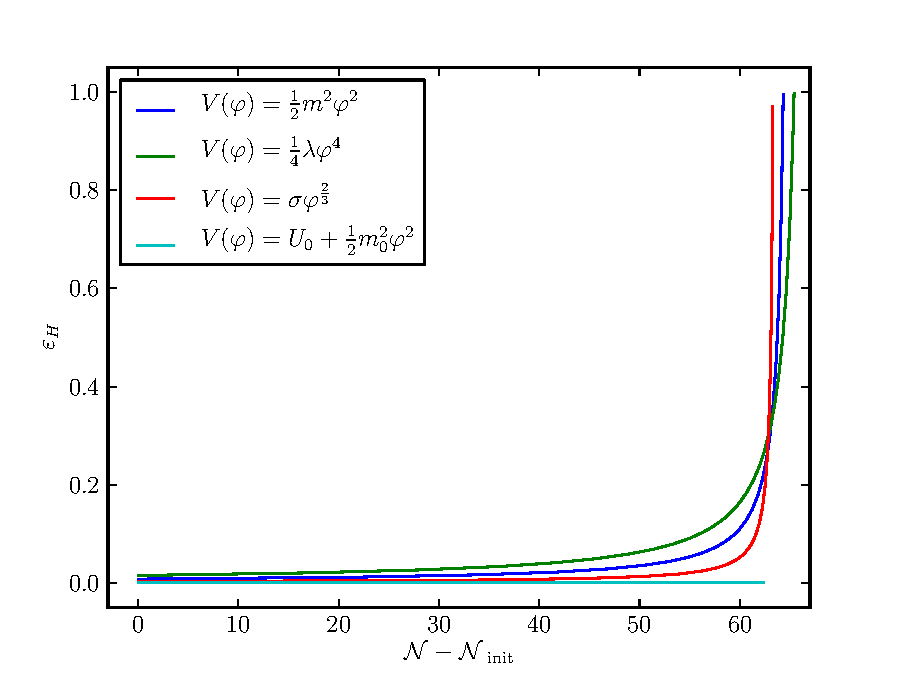
\includegraphics[width=0.75\textwidth]{numerical/graphs/epsilon_slowroll-large.pdf}
 % epsilon_slowroll-large.pdf: 432x324 pixel, 72dpi, 15.24x11.43 cm, bb=0 0 432 324
 \caption{The value of $\varepsilon_H$ for the four potentials.}
 \label{fig:eps-corr}
\end{figure}

\begin{figure}
 \centering
 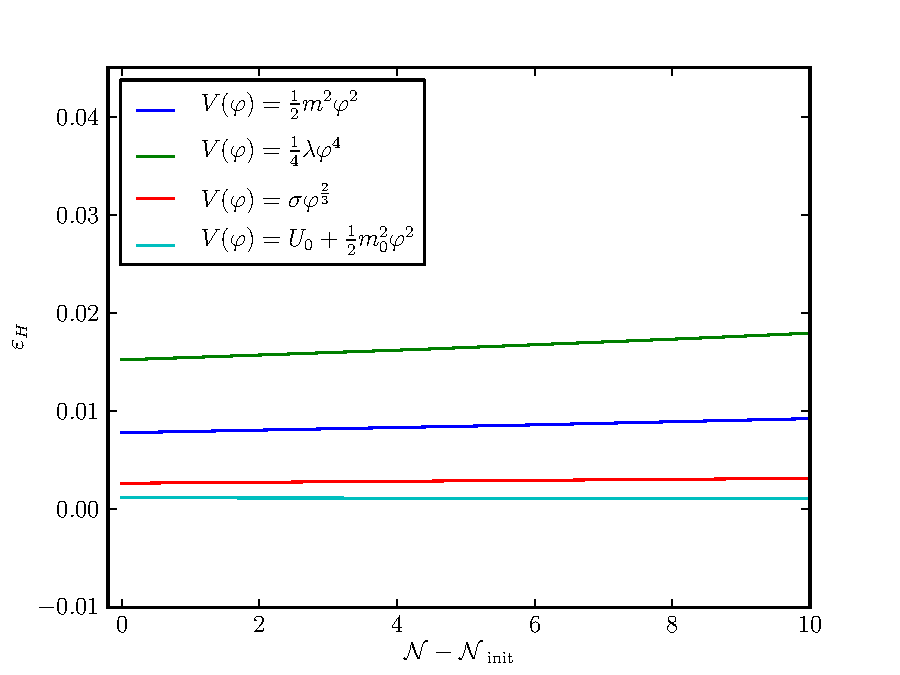
\includegraphics[width=0.75\textwidth]{numerical/graphs/epsilon_slowroll_zoom-large.pdf}
 % epsilon_slowroll-large.pdf: 432x324 pixel, 72dpi, 15.24x11.43 cm, bb=0 0 432 324
 \caption{The value of $\varepsilon_H$ for the four potentials at early times.}
 \label{fig:eps-zoom-corr}
\end{figure}

Figures~\ref{fig:eps-corr} and \ref{fig:eta-corr} show $\varepsilon_H$ and $\eta_H$ for the
four different models. Figures~\ref{fig:eps-zoom-corr} and
\ref{fig:eta-zoom-corr} show the early stages of the evolution as in
Fig~\ref{fig:cmp-src-zoom-kwmap}.

As is clear from these figures the change in the slow roll parameters is not easily related
to the differences in the profiles of the four potentials in Figure~\ref{fig:cmp-src-zoom-kwmap}. In
particular, although $\varepsilon_H$ and $\eta_H$ are quite different for the quadratic and quartic
models, the magnitude of $S$ after horizon crossing for these models is very similar.
\begin{figure}
 \centering
 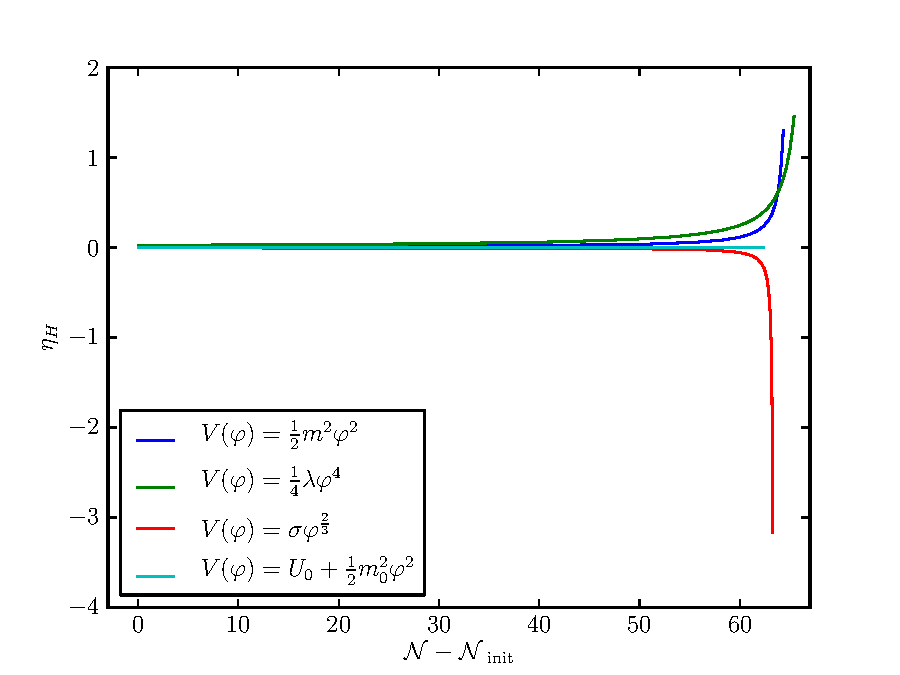
\includegraphics[width=0.75\textwidth]{numerical/graphs/eta_slowroll-large.pdf}
 % epsilon_slowroll-large.pdf: 432x324 pixel, 72dpi, 15.24x11.43 cm, bb=0 0 432 324
 \caption{The value of $\eta_H$ for the four potentials.}
 \label{fig:eta-corr}
\end{figure}

\begin{figure}
 \centering
 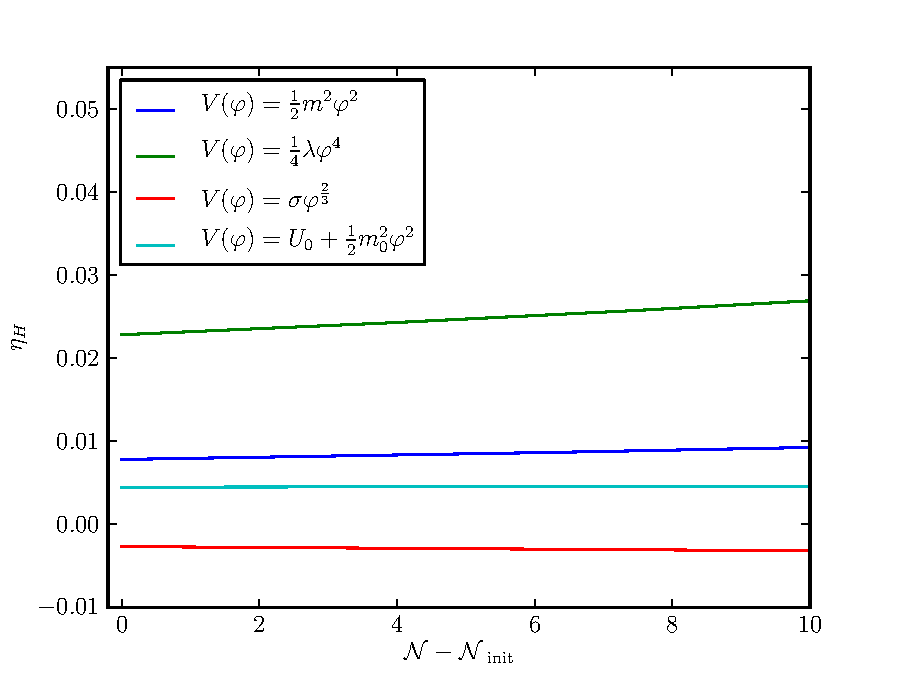
\includegraphics[width=0.75\textwidth]{numerical/graphs/eta_slowroll_zoom-large.pdf}
 % epsilon_slowroll-large.pdf: 432x324 pixel, 72dpi, 15.24x11.43 cm, bb=0 0 432 324
 \caption{The value of $\eta_H$ for the four potentials at early times.}
 \label{fig:eta-zoom-corr}
\end{figure}

At the earliest stages of the calculation of $S$, one or two e-foldings after the initialisation of
the first order perturbation, there appear to be small oscillations which affect the models in
different ways. The highly oscillatory initial conditions, combined with the small but appreciable
differences in $\varepsilon_H$ and $\eta_H$ contribute to this effect. In
Figure~\ref{fig:cos-keta-corr} the real part of the phase of the initial condition for $\dvp1$ is
plotted just after initialisation for the four potentials. The small differences in phase for each
model combined with the sharp cutoff at large and small $k$ values could explain the variations
in $|S|$ at early times as seen in Figure~\ref{fig:cmp-src-zoom-kwmap}. 

\begin{figure}
 \centering
 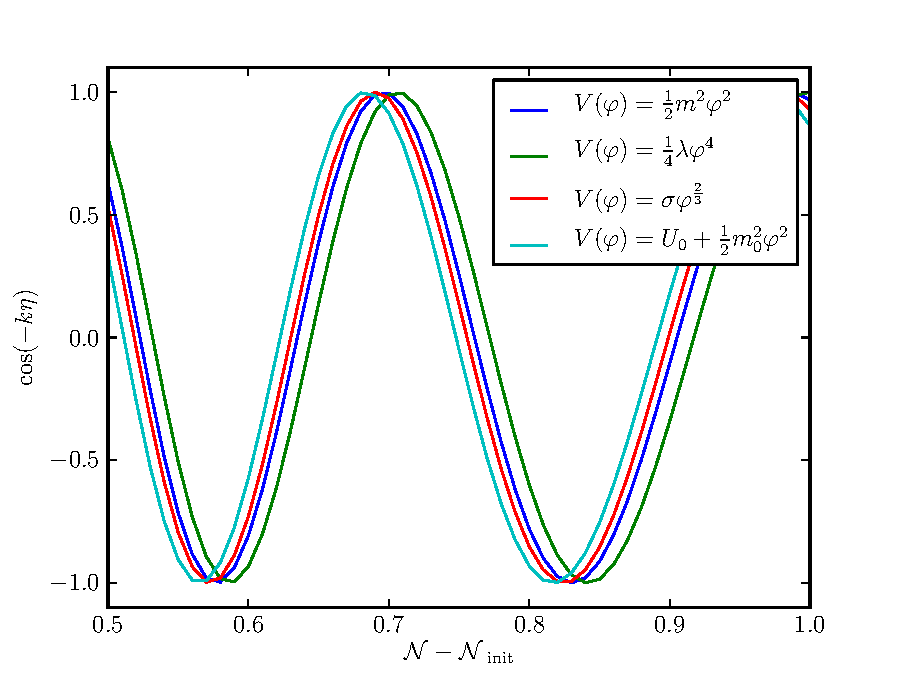
\includegraphics[width=0.75\textwidth]{numerical/graphs/cos_keta_kwmap_zoom-large.pdf}
 % cos_keta_kwmap_zoom-large.pdf: 432x324 pixel, 72dpi, 15.24x11.43 cm, bb=0 0 432 324
 \caption{The real part of the phase in the Bunch Davies initial conditions for the four different
potentials at early times.}
 \label{fig:cos-keta-corr}
\end{figure}

\subsection{Point 8: Compare analytic solution with results}
\textbf{Please refer to Point 15 above.}

\subsection{Point 9: Add more explanation for why code was developed, and explain how
you would calculate \texorpdfstring{$\fnl$}{fNL}}

\textbf{Explanation for code; Added to the discussion of the numerical code in Section~8.4 on Pg
138:}

Our numerical code evolves the second order perturbation itself and gives an insight into how this
field behaves through the full course of the inflationary era. This is in contrast to other
approaches which only consider the result for the three point function of the field, or
alternatively of the curvature perturbation.
% 
The computational system handles perturbations with scales both inside and outside the horizon. Any
effects of horizon crossing are visible and no assumptions need to be made about the form of the
solution inside the horizon.

The numerical code, when developed with the full equation, will not require any simplifying
assumptions about the form of the potential used. This allows models which are not amenable to
analytic analysis to be examined. Examples of models which require consideration beyond the slow
roll approximation include single field models with a step or other feature in the potential, and
multi-field double inflation models where the field values are roughly equal.


The code we have developed is also applicable in other physical circumstances. Beyond scalar
perturbations the form of the source term is similar in other interesting cosmological physics. 
The generation and evolution of non-Gaussian curvature perturbations is, of course, directly related
to the behaviour of the second order scalars as has been described in Section~\ref{sec:fnl-intro}
and Section~\ref{sec:observable-perts}. Investigating and classifying non-Gaussian signatures for
inflationary models is the main goal of our future work.

The generation of vorticity in a cosmological setting has physical parallels with the equations we
have studied. This second order effect arises through the vector perturbations which we have not
considered in this thesis. Vorticity in the early universe could also lead to the generation of
primordial magnetic fields, an area which is of increasing interest
\cite{Christopherson:2009bt,1950ZNatA...5...65B}.
% 
The wave equations for tensor mode perturbations also exhibit the same form as the scalar equations
with a source term at second order. The code we have developed could be modified to examine the
behaviour of gravitational waves in the early universe at second order.

% % % % % % % % % % % % % % % % % % % % % % % % % % % % % % 
\textbf{Discussion of calculation of $\fnl$; Added to Section~6.3 on Pg 93:}
% % % % % % % % % % % % % % % % % % % % % % % % % % % % % % 

To go beyond the local shape of the non-Gaussianity it is necessary to calculate the full
bispectrum of the perturbations. In practice the bispectrum of the curvature perturbation on
uniform density hypersurfaces, $\zeta$, is used in setting observational limits. At first order this
is simply related to the comoving curvature perturbation by $\zeta_1 = -\R_1$. At second order the
relationship is more complicated. For large scales outside the horizon, $\zeta_2$ can be related to
the field perturbations in real space using \cite{Malik:2005cy}
% 
\begin{equation}
 \zeta_2(x^i) = -\frac{\H}{\vp_0'}\dvp2(x^i) - \left[4 - 3\frac{(\vp_0')^2 - a^2\U}{(\vp_0')^2/2
+a^2\U} \right]\left(\frac{\H}{\vp_0'} \right)^2 \dvp1(x^i)^2\,. 
\end{equation}
% 
In Fourier space this again introduces a convolution integral of the first order perturbations.

The bispectrum of $\zeta$ is given by
% 
\begin{equation}
 \langle \zeta(\kb_1)\zeta(\kb_2)\zeta(\kb_3)\rangle = 
        (2\pi)^3 \delta(\kb_1+\kb_2+\kb_3) B(k_1,k_2,k_3)\,,
\end{equation}
% 
where translation invariance introduces the delta function. The $k$ dependence of the bispectrum 
is usually separated from an overall amplitude factor and considered as a shape function
$F(k_1,k_2,k_3)$. The bispectrum is then of the form \cite{Liguori:2010hx, Babich:2004gb}
% 
\begin{equation}
 \langle \zeta(\kb_1)\zeta(\kb_2)\zeta(\kb_3)\rangle = 
        A (2\pi)^3 \delta(\kb_1 + \kb_2 + \kb_3) F(k_1,k_2,k_3)\,,
\end{equation}
% 
and for a particular shape function $F$ the best estimator for $A$ when the non-Gaussianity is
small is given by \cite{Babich:2004gb}
% 
\begin{equation}
\label{eq:fnlampl-apx}
\hat{A} = \frac{\sum_{\kb_i} \zeta(\kb_1)\zeta(\kb_2)\zeta(\kb_3) F(k_1,k_2,k_3)/ 
                (\sigma^2_{k_1}\sigma^2_{k_2}\sigma^2_{k_3}) }
                {\sum_{\kb_i} F(k_1,k_2,k_3)^2/(\sigma^2_{k_1}\sigma^2_{k_2}\sigma^2_{k_3})} \,,
\end{equation}
% 
where $\sigma_{k_i}$ is the variance of the mode and the sums run over all the triangles in $k$
space subject. If $\kb_3$ is chosen to be the longest side of the triangle then the triangle
inequality enforces
% 
\begin{equation}
 k_3 \le k_1 + k_2\,.
\end{equation}
% 
\eq{eq:fnlampl-apx} provides a blueprint for how to evaluate the bispectrum in terms of a
particular given shape. To compare a primordial bispectrum with the observed temperature bispectrum
from the CMB it is necessary to construct the spherical harmonics of the bispectrum and use
transfer functions to relate the primordial values with the observed values. We have not
carried out this procedure in this thesis. However, one of the goals of our future work is to
undertake such a comparison of the numerically generated bispectrum with the observed quantity. 

As mentioned above, the shape most often used in comparisons with observations is the local shape
given by the
ansatz in \eq{eq:fnllocdefn-intro}. The expression for $F_\mathrm{local}$ is
\cite{Babich:2004gb, Komatsu:2010fb}
% 
\begin{equation}
 F_\mathrm{local}(k_1,k_2,k_3) = 2N\fnlloc \left(\frac{1}{k_1^3 k_2^3}
                                  +\frac{1}{k_2^3 k_3^3} + \frac{1}{k_1^3 k_3^3}\right) \,,
\end{equation}
% 
where the spectrum has been taken to be scale invariant and $N$ is a normalisation factor. 

This is not the only shape
that has been considered and, as we have seen, non-canonical inflationary actions generate a
bispectrum which is peaked
when the magnitudes of the $k$ modes are approximately equal. The form of $F$ for the equilateral
case is \cite{Komatsu:2010fb}
% 
\begin{multline}
 F_\mathrm{eq}(k_1,k_2,k_3) = 6 N \fnleq \left\{ -\frac{1}{k_1^3 k_2^3} -\frac{1}{k_2^3 k_3^3}
                                -\frac{1}{k_3^3 k_1^3}  \right.\\
                                \left.-\frac{2}{(k_1 k_2 k_3)^2}  + \left[ \frac{1}{k_1 k_2^2 k_3^3}
+ \mathrm{5 perms} \right]
                                \right\} \,.
\end{multline}
% 

A third form has been proposed which is nearly orthogonal to the other two shapes
\cite{Senatore:2009gt}. These shapes all have the property that they are separable functions of
each $k_i$ or can be constructed from these separable functions. This property eases analytic
calculations but clearly does not hold for generic shapes. 
% 
There has been a proposal to define the
shape of the bispectrum in terms of a set of basis vector shapes
\cite{Fergusson:2009nv,Liguori:2010hx}. This would remove the need for only separable shapes to be
considered and would allow for a straightforward analysis of the bispectrum from its primordial
value up to the observed bispectrum in the CMB. 

We have seen that the second order scalar perturbation is not the direct observable quantity of
interest. The bispectrum of the curvature perturbations, which contains a contribution from the
second order non-linear part, can be compared with observations either by use of various
shape functions or through a full analysis with transfer of the primordial values. A future goal of
our work is to compare the bispectrum obtained numerically with that from observations.



